\documentclass[10pt]{beamer}
\usetheme{CambridgeUS}
\usecolortheme{dolphin}

% Remove shadows and customize design
\setbeamertemplate{blocks}[rounded][shadow=false]
\setbeamertemplate{title page}[default][colsep=-4bp,rounded=true,shadow=false]
\setbeamertemplate{frametitle}[default][center,shadow=false]

% Customize colors
\definecolor{darkblue}{RGB}{25,25,112}
\definecolor{lightblue}{RGB}{173,216,230}
\setbeamercolor{structure}{fg=darkblue}
\setbeamercolor{frametitle}{bg=lightblue,fg=darkblue}
\setbeamercolor{title}{fg=darkblue}

% Remove navigation symbols
\setbeamertemplate{navigation symbols}{}

% Customize footline
\setbeamertemplate{footline}{
  \leavevmode%
  \hbox{%
  \begin{beamercolorbox}[wd=.3\paperwidth,ht=2.25ex,dp=1ex,center]{author in head/foot}%
    \usebeamerfont{author in head/foot}\insertshortauthor
  \end{beamercolorbox}%
  \begin{beamercolorbox}[wd=.4\paperwidth,ht=2.25ex,dp=1ex,center]{title in head/foot}%
    \usebeamerfont{title in head/foot}\insertshorttitle
  \end{beamercolorbox}%
  \begin{beamercolorbox}[wd=.3\paperwidth,ht=2.25ex,dp=1ex,right]{date in head/foot}%
    \usebeamerfont{date in head/foot}\insertshortdate{}\hspace*{2em}
    \insertframenumber{} / \inserttotalframenumber\hspace*{2ex} 
  \end{beamercolorbox}}%
  \vskip0pt%
}

% Essential packages
\usepackage{graphicx}
\usepackage{amsmath}
\usepackage{booktabs}
\usepackage{tikz}
\usetikzlibrary{positioning,calc}
\usepackage{pgfplots}
\pgfplotsset{compat=1.18}

% Better spacing and formatting
\setlength{\itemsep}{0.3em}
\setbeamertemplate{itemize items}[circle]
\setbeamertemplate{enumerate items}[default]
\setbeamerfont{frametitle}{size=\Large,series=\bfseries}
\setbeamerfont{framesubtitle}{size=\large}

% Fix overfull hbox warnings and improve layout
\setbeamersize{text margin left=0.8cm,text margin right=0.8cm}
\setlength{\parskip}{0.3em}
\setlength{\leftmargini}{1.2em}

% Title page information
\title[ML Traffic Management]{Machine Learning and IoT Based Traffic Management System}
\subtitle{Prioritizing Emergency Vehicles and Reducing Congestion}
\author[Alomgir \& Saied]{
    \textbf{Alomgir Hossain} \\
    \textbf{Saied Afnan} \\[0.5em]
    \small{Department of Computer Science and Engineering} \\
    \small{Shahjalal University of Science and Technology}
}
\institute[SUST]{
    Department of Computer Science and Engineering \\
    Shahjalal University of Science and Technology \\
    Sylhet-3114, Bangladesh
}
\date[July 2025]{\today}

\begin{document}

% Title slide
\begin{frame}[plain]
    \titlepage
\end{frame}

% Outline
\begin{frame}{Outline}
    \begin{itemize}
        \item \textbf{Problem Statement}
        \item \textbf{Research Objectives}  
        \item \textbf{Methodology}
        \item \textbf{Results}
        \item \textbf{Implementation Challenges}
        \item \textbf{Economic Impact}
        \item \textbf{Conclusions}
        \item \textbf{Future Work}
    \end{itemize}
\end{frame}

\section{Problem Statement}

\begin{frame}{Traffic Crisis in Dhaka}
    \begin{columns}
        \begin{column}{0.55\textwidth}
            \begin{itemize}
                \item \textbf{Severe Congestion}: Average vehicle speed drops to 4.8 km/h
                \item \textbf{Economic Impact}: \$3.8 billion annual cost
                \item \textbf{Emergency Delays}: 56\% of emergency responses delayed
                \item \textbf{Infrastructure Limits}: Roads designed for smaller population
                \item \textbf{Mixed Traffic}: Complex vehicle types competing for space
            \end{itemize}
            
            \vspace{0.4cm}
            \begin{center}
                \textcolor{red}{\large\textbf{Need for Intelligent Traffic Management}}
            \end{center}
        \end{column}
        \begin{column}{0.45\textwidth}
            \begin{figure}[h]
                \centering
                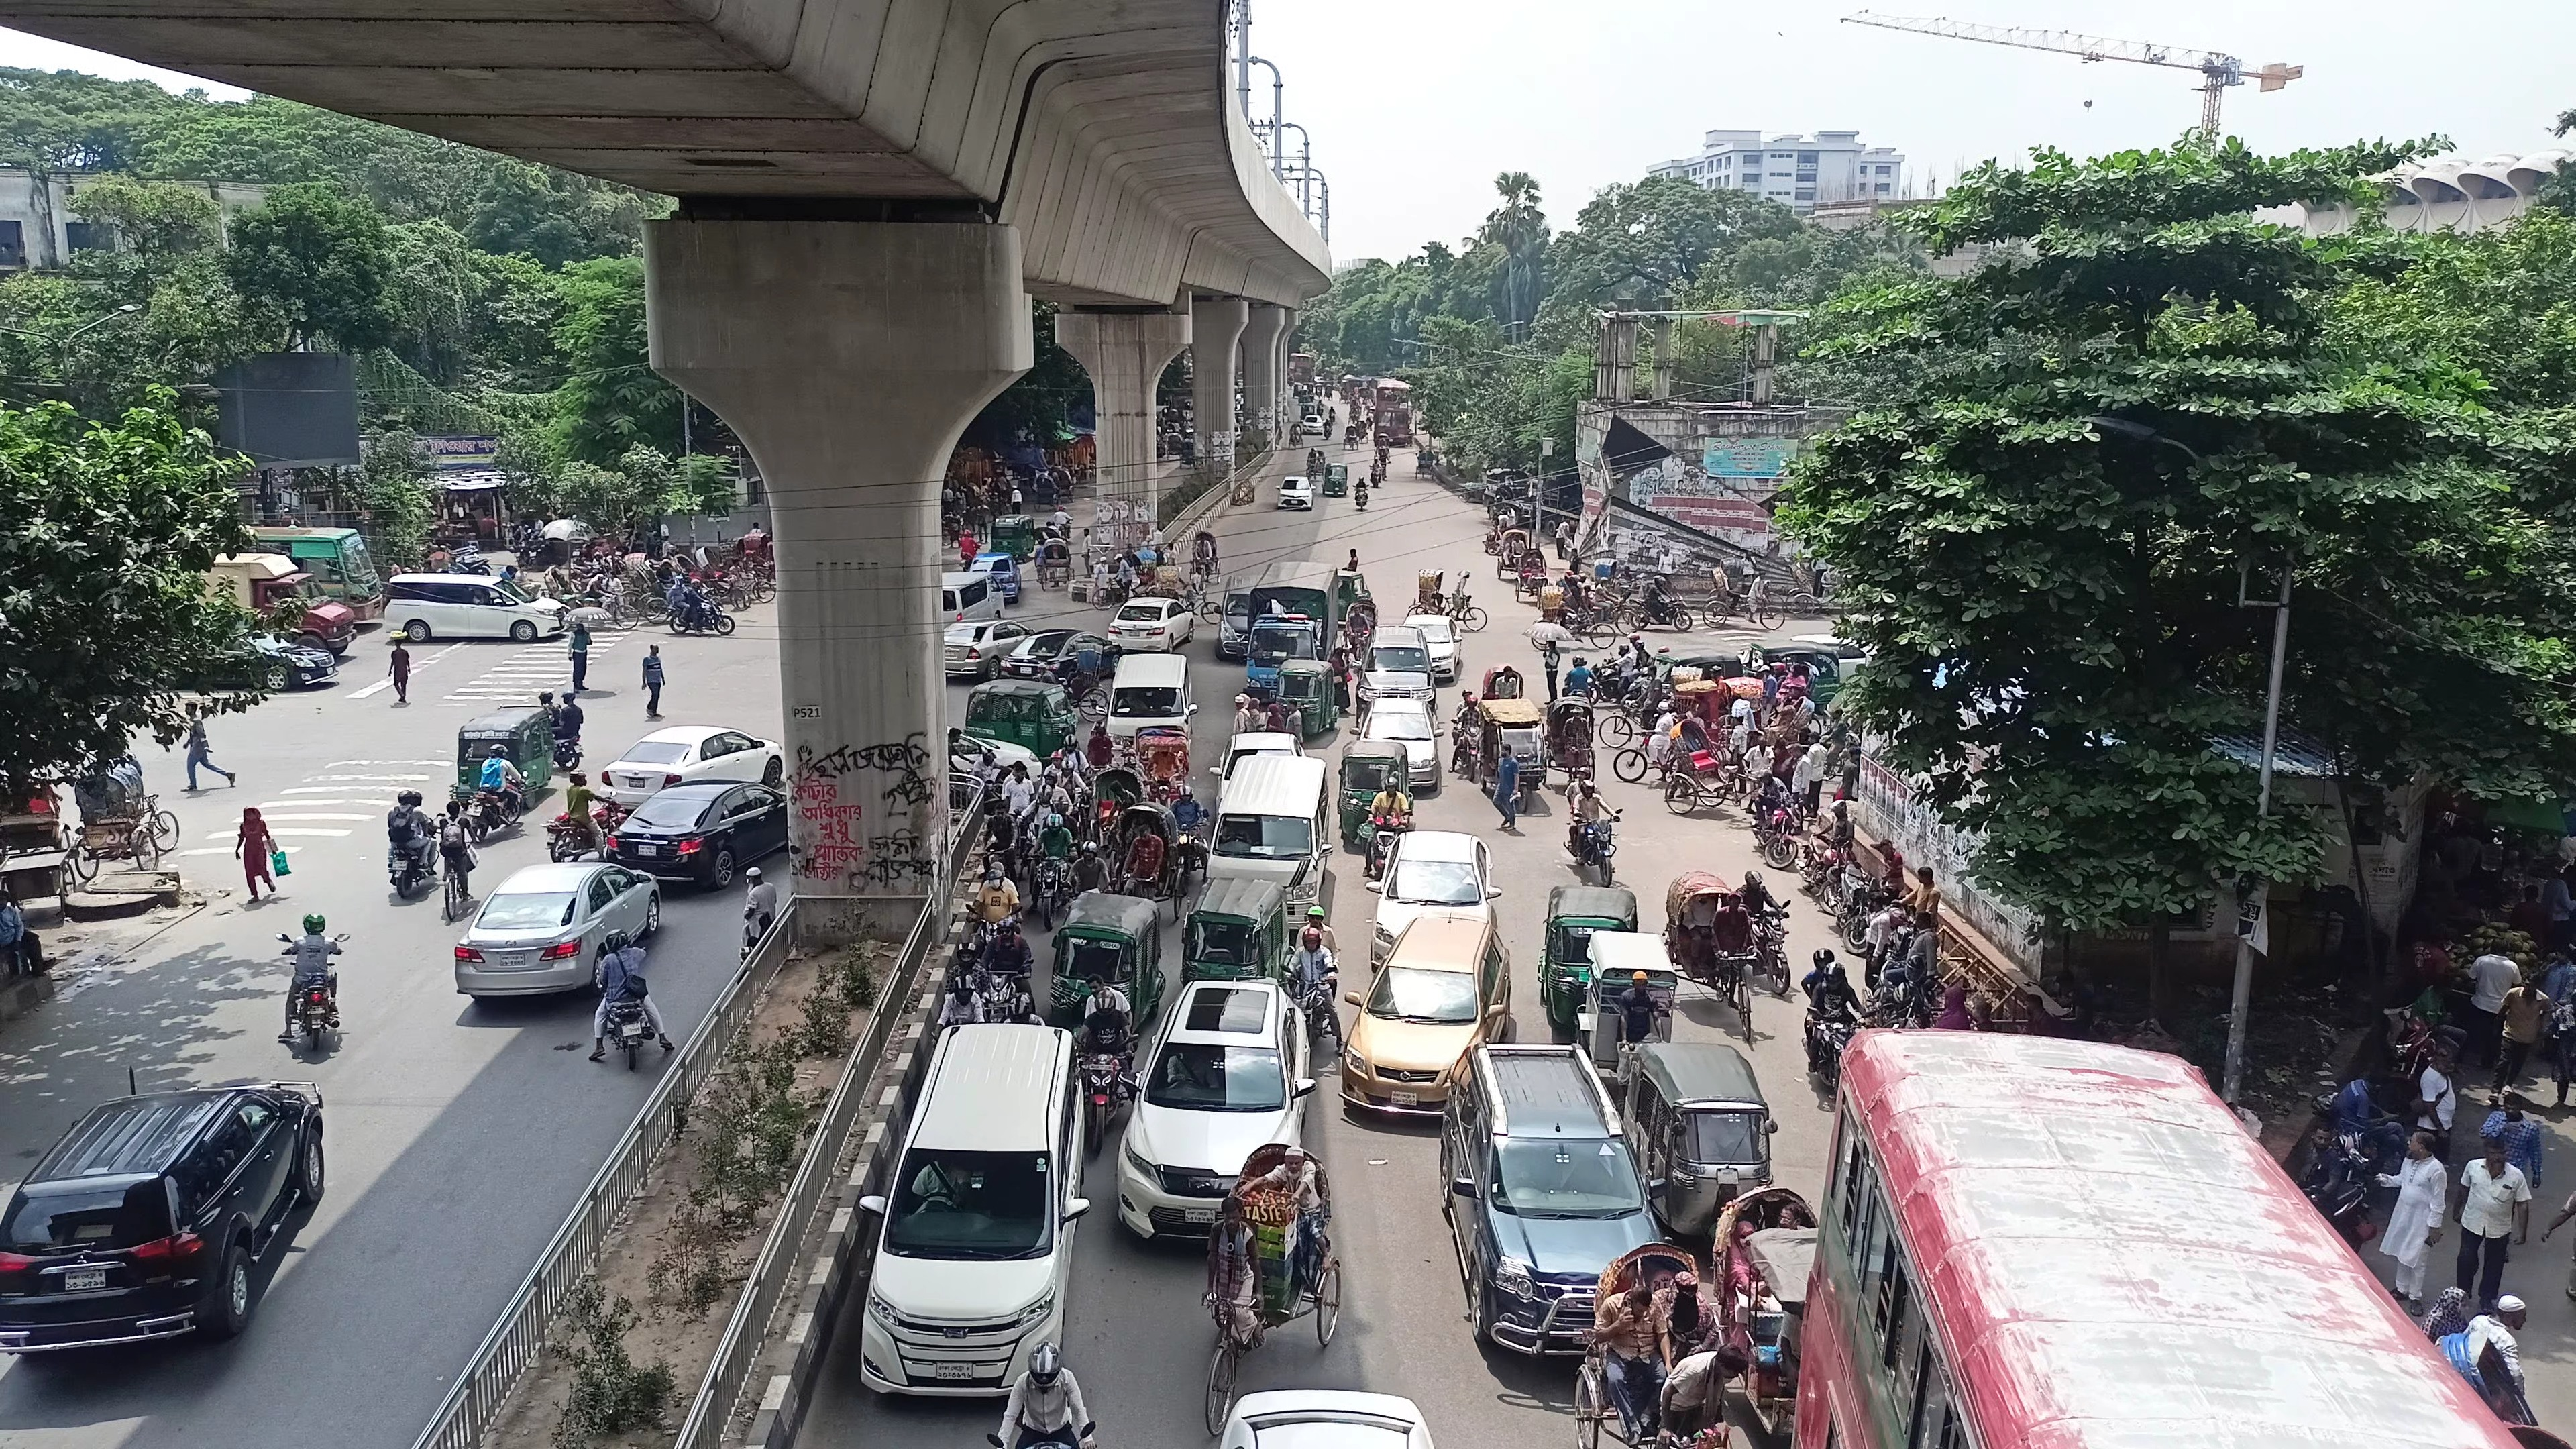
\includegraphics[width=\textwidth]{thesis_final/figures/shahabag.jpg}
                \caption{\footnotesize Shahbag Traffic Congestion}
            \end{figure}
        \end{column}
    \end{columns}
\end{frame}

\begin{frame}{Current Traffic Management Challenges}
    \begin{columns}
        \begin{column}{0.45\textwidth}
            \textbf{Technical Challenges:}
            \begin{itemize}
                \item Fixed timing signals
                \item No real-time adaptation
                \item Manual traffic control
                \item Limited sensor integration
                \item Poor emergency prioritization
            \end{itemize}
            
            \vspace{0.3cm}
            \textbf{Impact on Society:}
            \begin{itemize}
                \item 22 million population affected
                \item Daily productivity losses
                \item Increased fuel consumption
                \item Emergency service delays
            \end{itemize}
        \end{column}
        \begin{column}{0.55\textwidth}
            \begin{figure}[h]
                \centering
                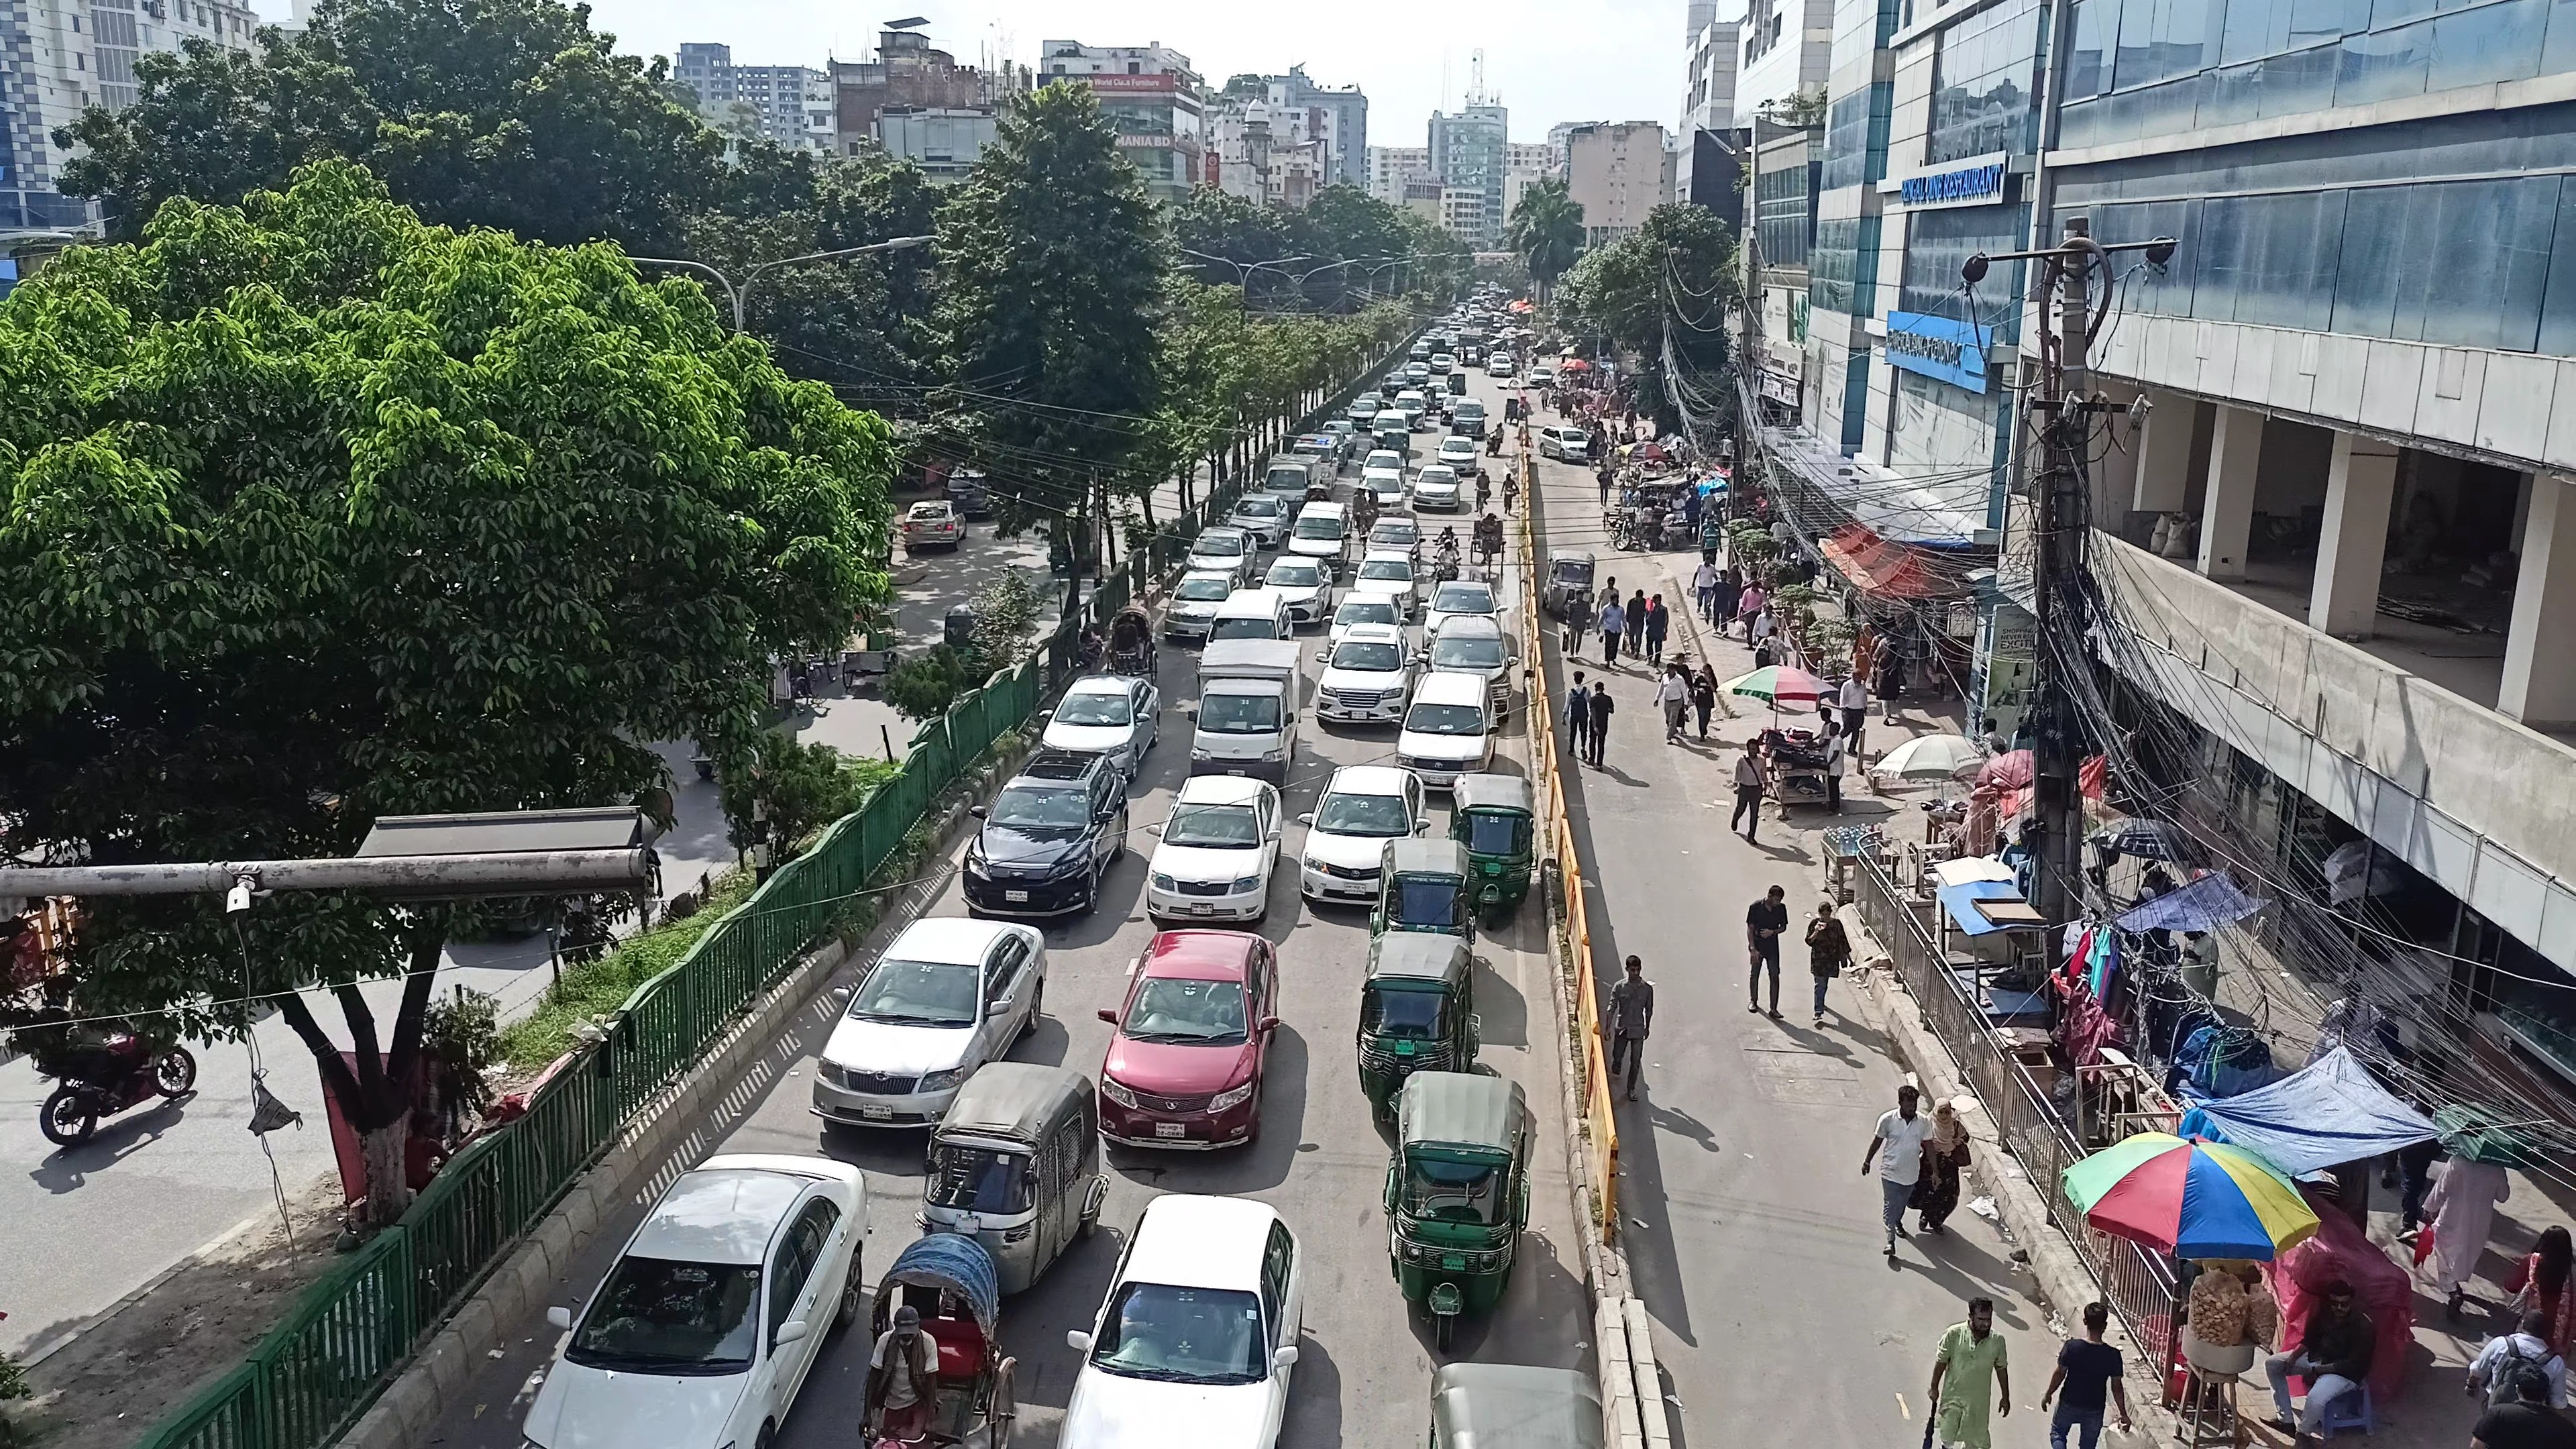
\includegraphics[width=0.47\textwidth]{thesis_final/figures/kawran_bazar.jpg}
                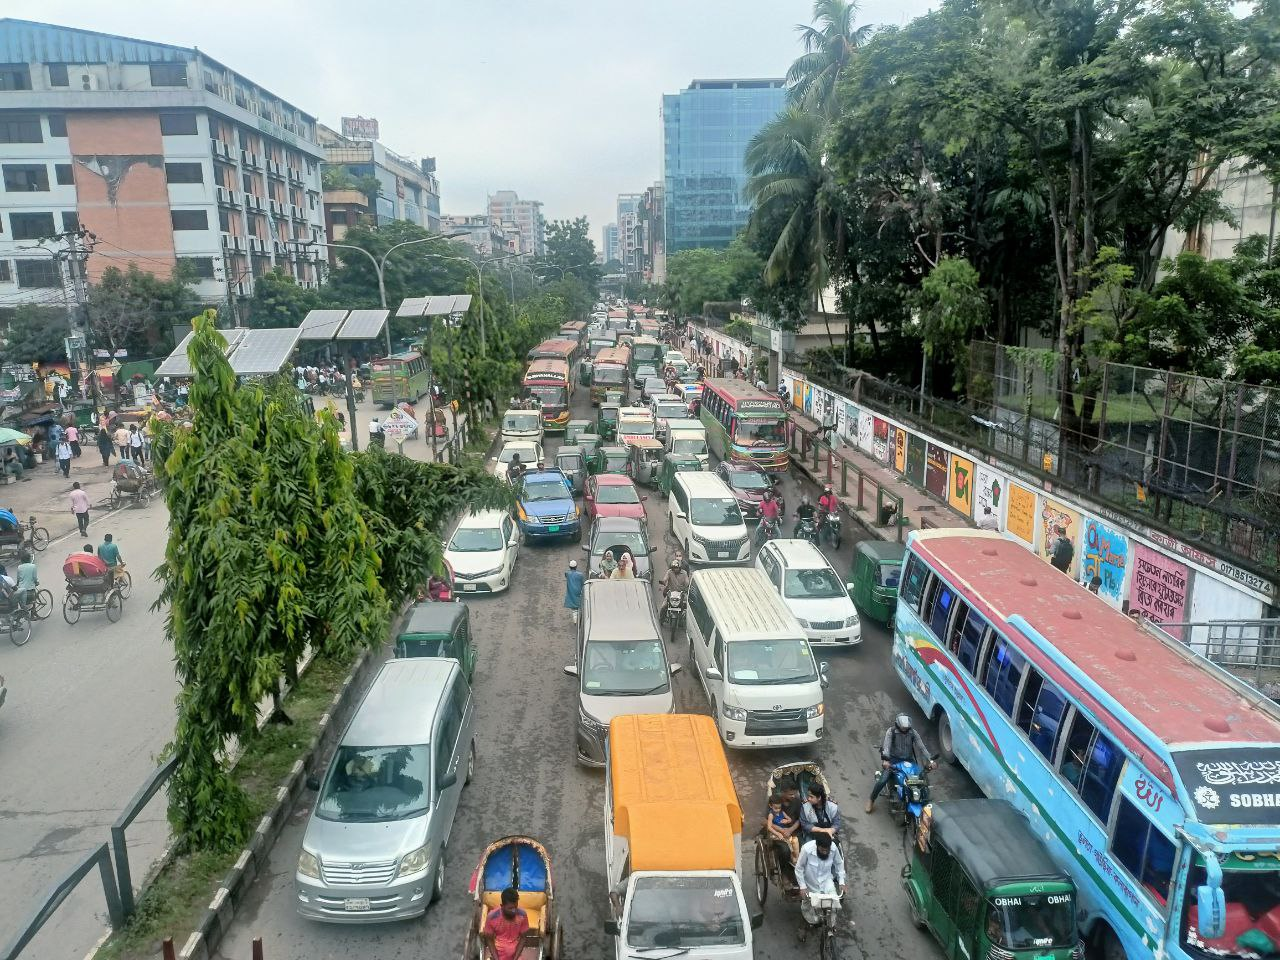
\includegraphics[width=0.47\textwidth]{thesis_final/figures/science_lab.jpg}
                \caption{\footnotesize Traffic Congestion at Major Intersections}
            \end{figure}
        \end{column}
    \end{columns}
    
    \vspace{0.4cm}
    \begin{center}
        \textcolor{blue}{\large\textbf{Traditional systems cannot handle dynamic traffic patterns}}
    \end{center}
\end{frame}

\begin{frame}{Research Motivation}
    \begin{columns}
        \begin{column}{0.6\textwidth}
            \begin{enumerate}
                \item \textbf{Urbanization Crisis}
                \begin{itemize}
                    \item Population growth exceeds infrastructure development
                    \item Vehicle ownership increasing exponentially
                \end{itemize}
                
                \item \textbf{Technology Opportunity}
                \begin{itemize}
                    \item IoT and ML technologies are now mature
                    \item Real-time processing capabilities available
                \end{itemize}
                
                \item \textbf{Life-Critical Need}
                \begin{itemize}
                    \item Emergency services facing critical delays
                    \item Traffic accidents on the rise
                \end{itemize}
                
                \item \textbf{Economic Necessity}
                \begin{itemize}
                    \item Massive economic losses due to traffic
                    \item Cost-effective solutions needed
                \end{itemize}
            \end{enumerate}
        \end{column}
        \begin{column}{0.4\textwidth}
            \begin{figure}[h]
                \centering
                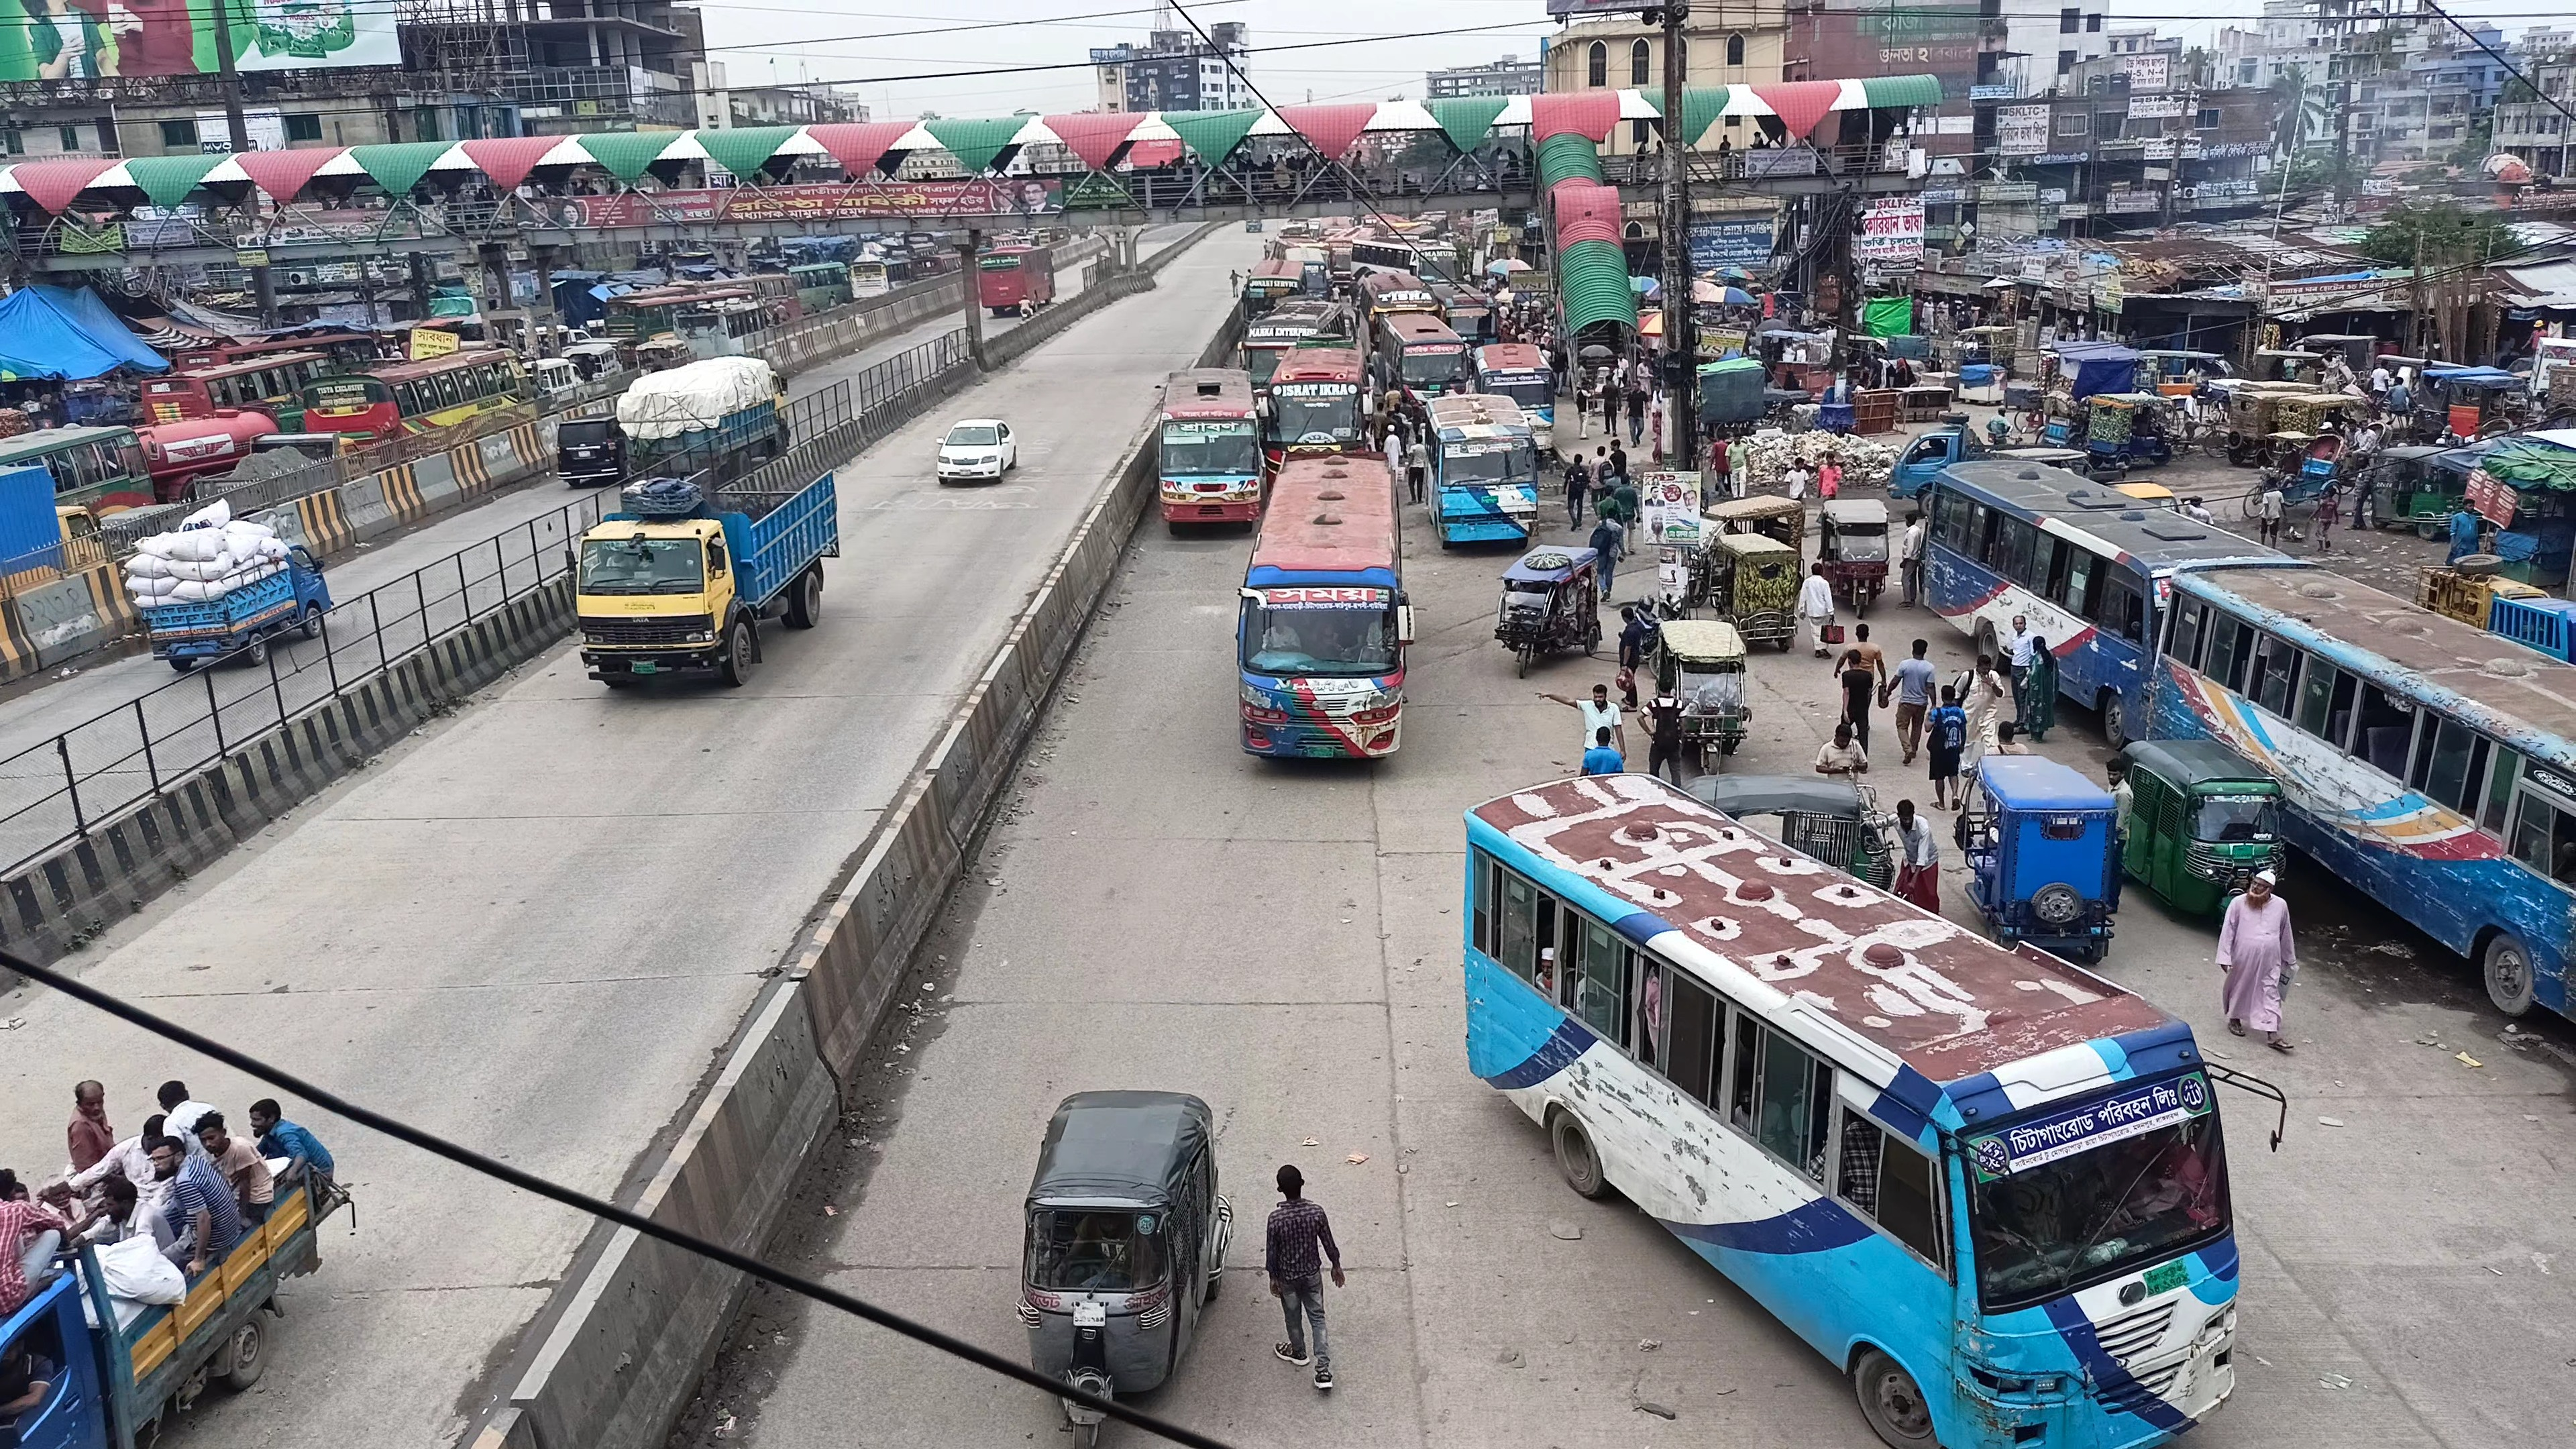
\includegraphics[width=0.9\textwidth]{thesis_final/figures/narayanganj.jpg}
                \caption{Traffic Scenario in Narayanganj}
            \end{figure}
        \end{column}
    \end{columns}
\end{frame}

\section{Research Objectives}

\begin{frame}{Key Objectives}
    \begin{columns}
        \begin{column}{0.6\textwidth}
            \begin{enumerate}
                \item \textbf{Real-time Vehicle Detection}
                \begin{itemize}
                    \item YOLOv11 based object detection
                    \item Classify vehicles, pedestrians, emergency vehicles
                \end{itemize}
                
                \item \textbf{Emergency Vehicle Prioritization}
                \begin{itemize}
                    \item Automatic detection and signal adjustment
                    \item Reduce emergency response times
                \end{itemize}
                
                \item \textbf{Adaptive Traffic Control}
                \begin{itemize}
                    \item Dynamic signal timing based on traffic density
                    \item Prevent lane starvation
                \end{itemize}
                
                \item \textbf{IoT Integration}
                \begin{itemize}
                    \item Arduino, Raspberry Pi, NodeMCU
                    \item Connect ML algorithms with physical infrastructure
                \end{itemize}
            \end{enumerate}
        \end{column}
        \begin{column}{0.4\textwidth}
            \begin{figure}[h]
                \centering
                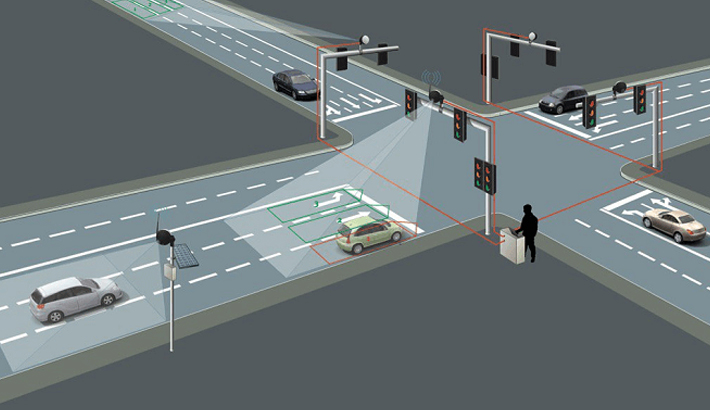
\includegraphics[width=0.9\textwidth]{thesis_final/figures/cctv.jpg}
                \caption{CCTV Infrastructure}
            \end{figure}
        \end{column}
    \end{columns}
\end{frame}

\section{Methodology}

\begin{frame}{Research Methodology Overview}
    \begin{center}
        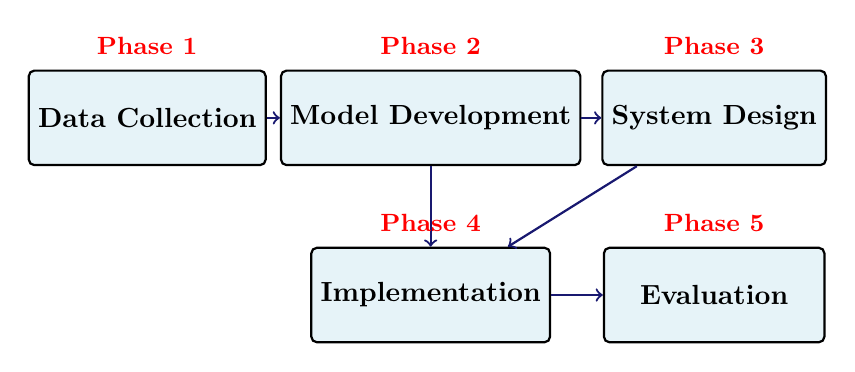
\begin{tikzpicture}[
            scale=0.9,
            box/.style={draw, rectangle, minimum width=2.8cm, minimum height=1.2cm, 
                       fill=lightblue!30, rounded corners=2pt, thick},
            arrow/.style={->, thick, color=darkblue}
        ]
            \node[box] (data) at (0,2.5) {\textbf{Data Collection}};
            \node[box] (model) at (4,2.5) {\textbf{Model Development}};
            \node[box] (system) at (8,2.5) {\textbf{System Design}};
            \node[box] (impl) at (4,0) {\textbf{Implementation}};
            \node[box] (eval) at (8,0) {\textbf{Evaluation}};
            
            \draw[arrow] (data) -- (model);
            \draw[arrow] (model) -- (system);
            \draw[arrow] (system) -- (impl);
            \draw[arrow] (impl) -- (eval);
            \draw[arrow] (model) -- (impl);
            
            % Add phase numbers
            \node[above=2pt of data] {\small\textcolor{red}{\textbf{Phase 1}}};
            \node[above=2pt of model] {\small\textcolor{red}{\textbf{Phase 2}}};
            \node[above=2pt of system] {\small\textcolor{red}{\textbf{Phase 3}}};
            \node[above=2pt of impl] {\small\textcolor{red}{\textbf{Phase 4}}};
            \node[above=2pt of eval] {\small\textcolor{red}{\textbf{Phase 5}}};
        \end{tikzpicture}
    \end{center}
    
    \vspace{0.5cm}
    \textbf{5-Phase Systematic Approach:}
    \begin{itemize}
        \item Phase 1: Comprehensive traffic data collection from 7 strategic locations
        \item Phase 2: YOLOv11 model training and optimization
        \item Phase 3: IoT-based system architecture design
        \item Phase 4: Real-world pilot deployment
        \item Phase 5: Performance evaluation and analysis
    \end{itemize}
\end{frame}

\begin{frame}{Data Collection Strategy}
    \begin{columns}
        \begin{column}{0.5\textwidth}
            \textbf{Strategic Locations:}
            \begin{enumerate}
                \item Shahbag (Academic area)
                \item Polton (Residential/Commercial)
                \item Motijheel (Business district)
                \item Science Lab (Transit hub)
                \item Panthapath (Major arterial)
                \item Bijoy Sarani (North-South corridor)
                \item Gulistan (Dense urban area)
            \end{enumerate}
        \end{column}
        \begin{column}{0.5\textwidth}
            \textbf{Data Characteristics:}
            \begin{itemize}
                \item 6-month collection period
                \item Multiple time periods
                \item Various weather conditions
                \item High-resolution imagery
                \item Diverse traffic scenarios
            \end{itemize}
            
            \vspace{0.3cm}
            \textbf{Quality Assurance:}
            \begin{itemize}
                \item Multi-level annotation review
                \item Expert domain validation
                \item Consistency checks
                \item Data augmentation techniques
            \end{itemize}
        \end{column}
    \end{columns}
\end{frame}

\begin{frame}{System Architecture}
    \begin{center}
        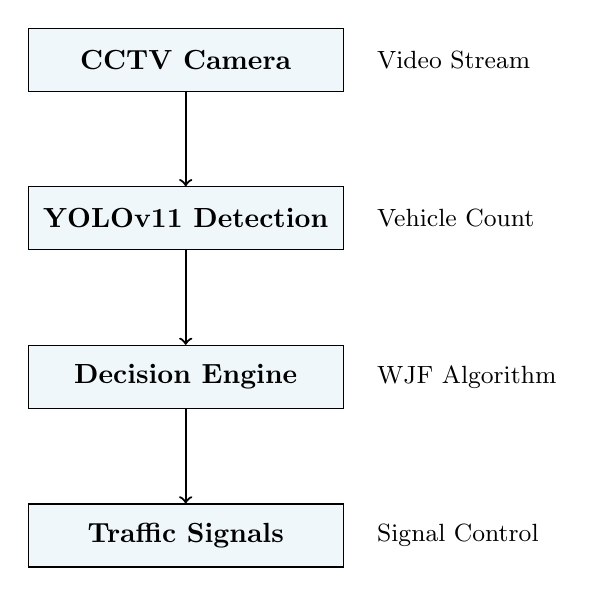
\begin{tikzpicture}[
            node distance=1.2cm,
            box/.style={rectangle, draw, minimum width=4cm, minimum height=0.8cm, 
                       fill=lightblue!20, align=center},
            arrow/.style={->, thick}
        ]
            % Simple vertical flow
            \node[box] (camera) {\textbf{CCTV Camera}};
            \node[box, below=of camera] (detection) {\textbf{YOLOv11 Detection}};
            \node[box, below=of detection] (decision) {\textbf{Decision Engine}};
            \node[box, below=of decision] (control) {\textbf{Traffic Signals}};
            
            % Simple arrows
            \draw[arrow] (camera) -- (detection);
            \draw[arrow] (detection) -- (decision);
            \draw[arrow] (decision) -- (control);
            
            % Simple side labels
            \node[right=0.3cm] at (camera.east) {\small Video Stream};
            \node[right=0.3cm] at (detection.east) {\small Vehicle Count};
            \node[right=0.3cm] at (decision.east) {\small WJF Algorithm};
            \node[right=0.3cm] at (control.east) {\small Signal Control};
        \end{tikzpicture}
    \end{center}
\end{frame}

\begin{frame}{YOLOv11 Model Architecture}
    \begin{columns}
        \begin{column}{0.5\textwidth}
            \textbf{Why YOLOv11?}
            \begin{itemize}
                \item Real-time processing capability
                \item Superior accuracy vs previous versions
                \item Efficient memory usage
                \item Multi-scale object detection
                \item Robust performance in challenging conditions
            \end{itemize}
            
            \vspace{0.3cm}
            \textbf{Model Specifications:}
            \begin{itemize}
                \item Input: 640x640 pixels
                \item Backbone: CSPDarkNet53
                \item Neck: PANet
                \item Head: YOLOv11 Detection Head
            \end{itemize}
        \end{column}
        \begin{column}{0.5\textwidth}
            \begin{figure}[h]
                \centering
                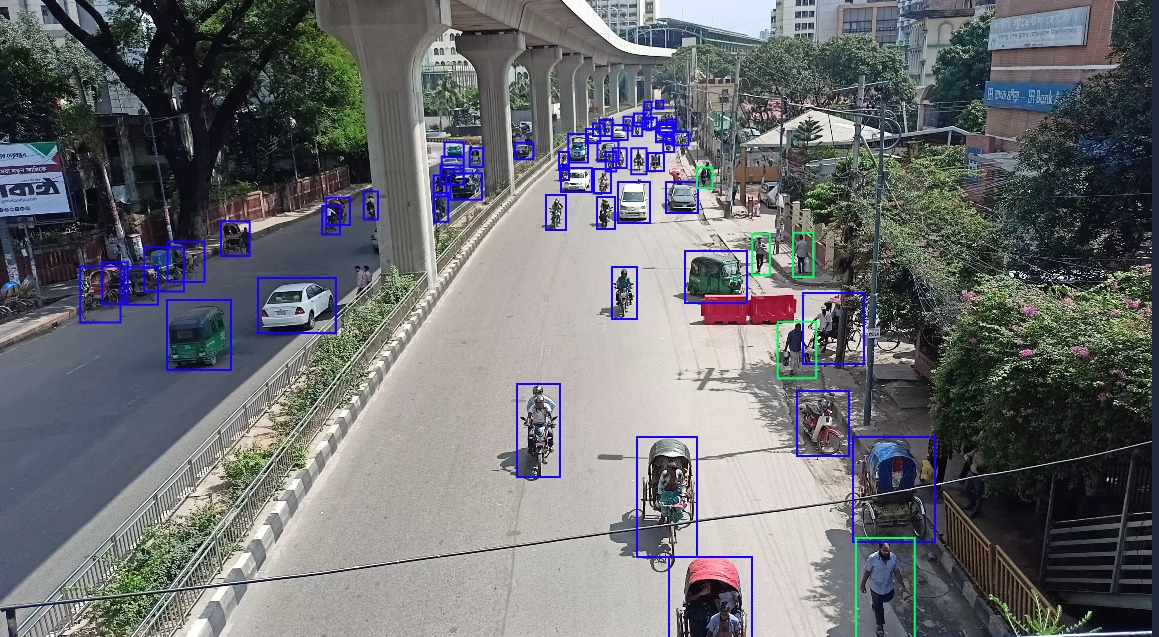
\includegraphics[width=0.9\textwidth]{thesis_final/figures/annotated.jpg}
                \caption{YOLOv11 Detection Example}
            \end{figure}
            
            \textbf{Training Details:}
            \begin{table}[h]
                \tiny
                \begin{tabular}{|l|l|}
                    \hline
                    \textbf{Parameter} & \textbf{Value} \\
                    \hline
                    Model & YOLOv11m \\
                    Epochs & 256 \\
                    Batch Size & 16 \\
                    Learning Rate & 0.01 \\
                    Optimizer & AdamW \\
                    \hline
                \end{tabular}
            \end{table}
        \end{column}
    \end{columns}
\end{frame}

\begin{frame}{Dataset and Training}
    \begin{columns}
        \begin{column}{0.5\textwidth}
            \textbf{Dataset Statistics:}
            \begin{itemize}
                \item 3,784 images collected
                \item 171,436 annotated objects
                \item 7 strategic locations
                \item 21 vehicle categories
            \end{itemize}
            
            \vspace{0.5cm}
            \textbf{Training Configuration:}
            \begin{itemize}
                \item YOLOv11m model
                \item 256 epochs
                \item 640x640 resolution
                \item AdamW optimizer
            \end{itemize}
        \end{column}
        \begin{column}{0.5\textwidth}
            \begin{figure}[h]
                \centering
                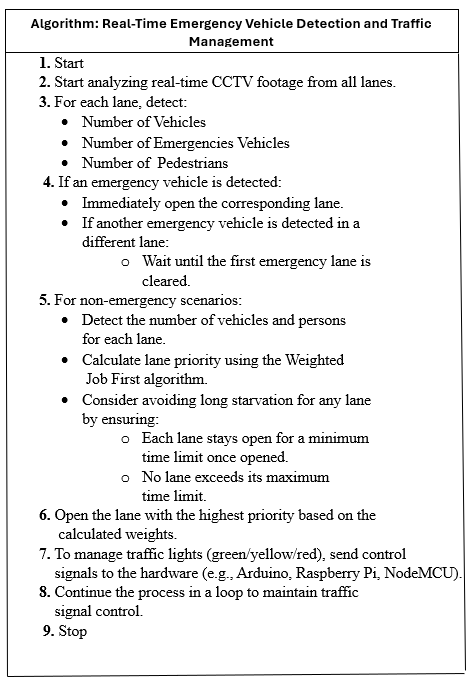
\includegraphics[width=0.9\textwidth]{thesis_final/figures/10.png}
                \caption{Training Progress}
            \end{figure}
            
            \begin{table}[h]
                \scriptsize
                \caption{Object Distribution}
                \begin{tabular}{|l|c|}
                    \hline
                    \textbf{Category} & \textbf{Count} \\
                    \hline
                    Regular Vehicles & 107,004 \\
                    Pedestrians & 63,541 \\
                    Emergency Vehicles & 781 \\
                    \hline
                    \textbf{Total} & \textbf{171,436} \\
                    \hline
                \end{tabular}
            \end{table}
        \end{column}
    \end{columns}
\end{frame}

\section{Results}

\begin{frame}{Model Performance Overview}
    \begin{columns}
        \begin{column}{0.5\textwidth}
            \textbf{Detection Accuracy:}
            \begin{itemize}
                \item \textbf{Overall mAP50}: 79\%
                \item \textbf{Vehicle Detection}: 85\%
                \item \textbf{Pedestrian Detection}: 82\%
                \item \textbf{Emergency Vehicle}: 85\%
            \end{itemize}
            
            \vspace{0.3cm}
            \textbf{System Performance:}
            \begin{itemize}
                \item \textbf{Response Time}: 222ms avg
                \item \textbf{System Uptime}: 98.9\%
                \item \textbf{Processing Rate}: 30+ FPS
                \item \textbf{Memory Usage}: 2.1GB
            \end{itemize}
        \end{column}
        \begin{column}{0.5\textwidth}
            \begin{figure}[h]
                \centering
                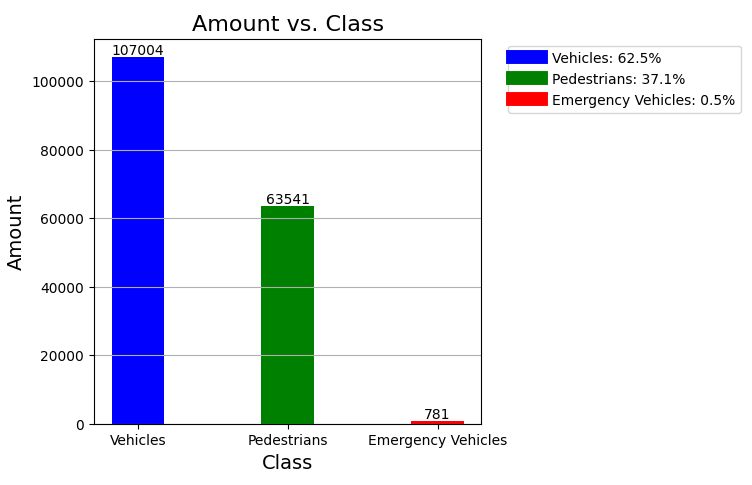
\includegraphics[width=0.9\textwidth]{thesis_final/figures/11.png}
                \caption{Performance Metrics}
            \end{figure}
            
            \begin{center}
                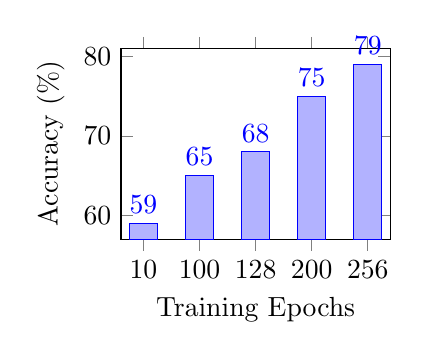
\begin{tikzpicture}
                    \begin{axis}[
                        ybar,
                        width=5cm,
                        height=4cm,
                        ylabel={Accuracy (\%)},
                        symbolic x coords={10,100,128,200,256},
                        xlabel={Training Epochs},
                        xtick=data,
                        nodes near coords,
                        nodes near coords align={vertical},
                    ]
                    \addplot coordinates {
                        (10,59)
                        (100,65)
                        (128,68)
                        (200,75)
                        (256,79)
                    };
                    \end{axis}
                \end{tikzpicture}
            \end{center}
        \end{column}
    \end{columns}
\end{frame}

\begin{frame}{Confusion Matrix Analysis}
    \begin{columns}
        \begin{column}{0.5\textwidth}
            \begin{figure}[h]
                \centering
                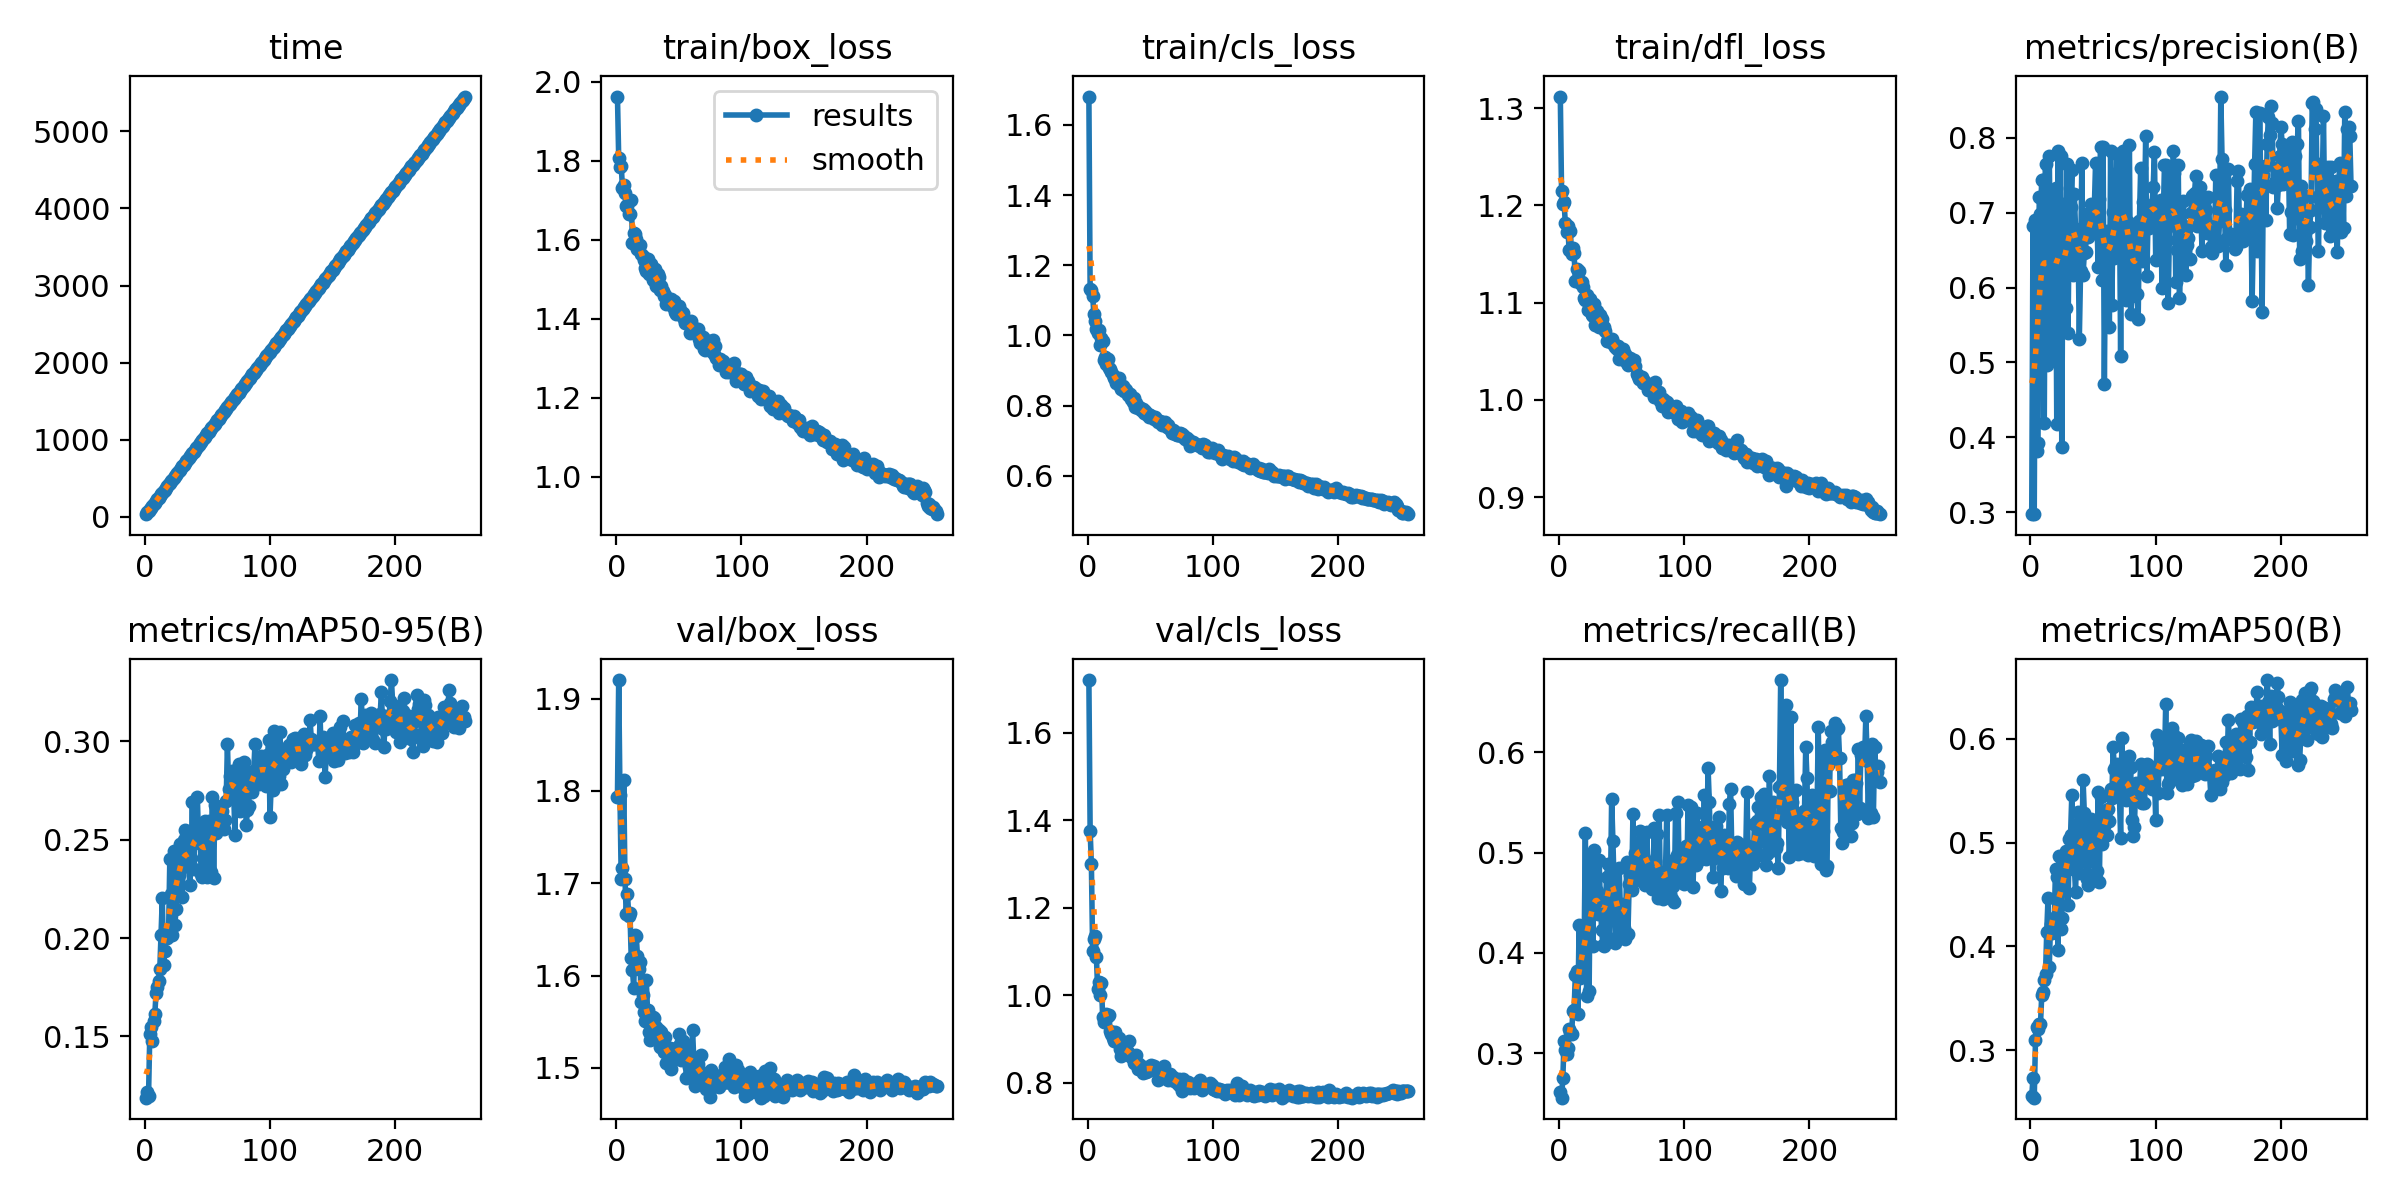
\includegraphics[width=0.9\textwidth]{thesis_final/figures/13.png}
                \caption{Confusion Matrix Visualization}
            \end{figure}
        \end{column}
        \begin{column}{0.5\textwidth}
            \begin{table}[h]
                \scriptsize
                \caption{Model Confusion Matrix}
                \begin{tabular}{|l|c|c|c|c|}
                    \hline
                    \textbf{True/Pred} & \textbf{Emerg} & \textbf{Person} & \textbf{Vehicle} & \textbf{BG} \\
                    \hline
                    Emergency & \textbf{4} & 3 & 0 & 1 \\
                    Person & 0 & \textbf{2080} & 47 & 890 \\
                    Vehicle & 0 & 41 & \textbf{4111} & 1191 \\
                    Background & 0 & 1152 & 0 & \textbf{1222} \\
                    \hline
                \end{tabular}
            \end{table}
            
            \textbf{Performance Metrics:}
            \begin{itemize}
                \item \textbf{Precision}: 83.2\%
                \item \textbf{Recall}: 81.7\%
                \item \textbf{F1-Score}: 82.4\%
                \item \textbf{Training Time}: 45.6 hours
            \end{itemize}
        \end{column}
    \end{columns}
\end{frame}

\begin{frame}{Performance Improvements}
    \begin{columns}
        \begin{column}{0.5\textwidth}
            \begin{table}[h]
                \tiny
                \caption{Traffic Flow Improvements}
                \begin{tabular}{|l|c|c|c|}
                    \hline
                    \textbf{Metric} & \textbf{Traditional} & \textbf{Proposed} & \textbf{Improvement} \\
                    \hline
                    Wait Time & 12.5 min & 8.4 min & \textcolor{green}{\textbf{33\% ↓}} \\
                    Emergency & 8.5 min & 3.7 min & \textcolor{green}{\textbf{56\% ↓}} \\
                    Lane Util. & 70\% & 92\% & \textcolor{green}{\textbf{31\% ↑}} \\
                    Starvation & 3.2/hr & 0.1/hr & \textcolor{green}{\textbf{97\% ↓}} \\
                    \hline
                \end{tabular}
            \end{table}
        \end{column}
        \begin{column}{0.5\textwidth}
            \begin{figure}[h]
                \centering
                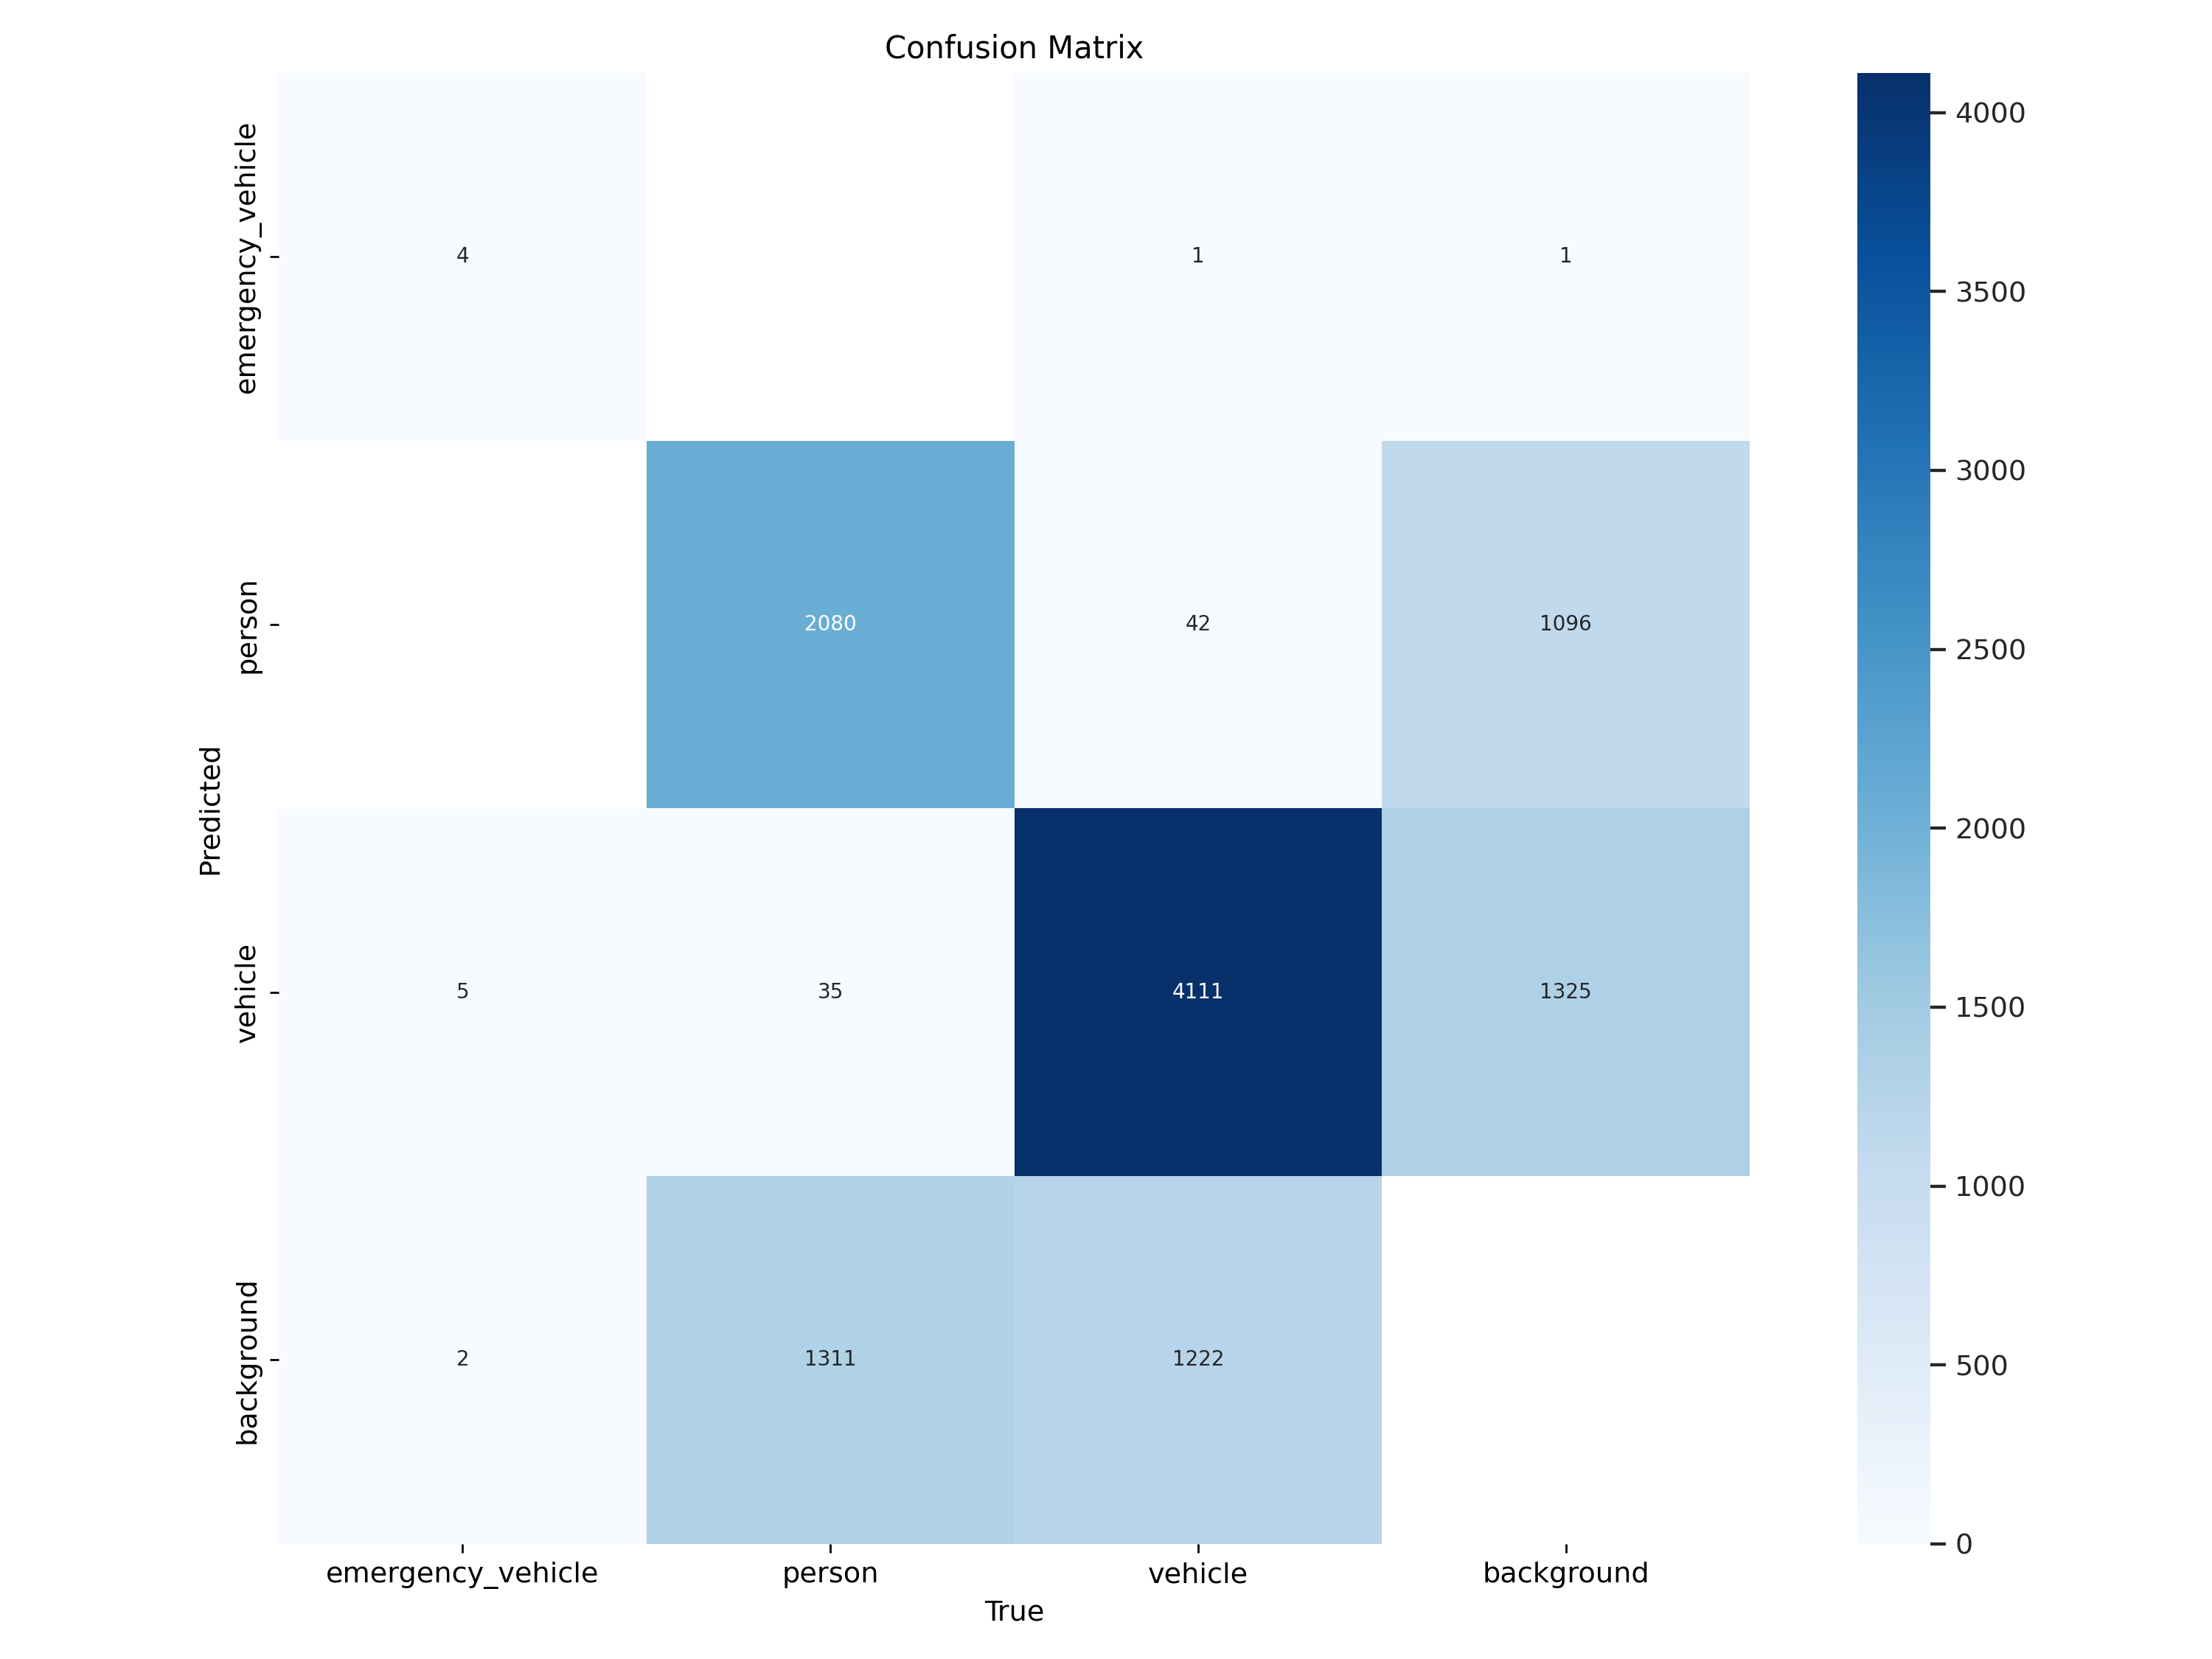
\includegraphics[width=0.9\textwidth]{thesis_final/figures/14.png}
                \caption{Performance Comparison}
            \end{figure}
        \end{column}
    \end{columns}
    
    \vspace{0.5cm}
    \begin{center}
        \textcolor{blue}{\textbf{Significant improvements in all key metrics}}
    \end{center}
\end{frame}

\begin{frame}{Real-World Deployment Results}
    \begin{columns}
        \begin{column}{0.5\textwidth}
            \textbf{Pilot Locations:}
            \begin{enumerate}
                \item Shahbag Intersection
                \item Motijheel Commercial Area
                \item Science Lab Junction
            \end{enumerate}
            
            \vspace{0.3cm}
            \textbf{Deployment Duration:}
            \begin{itemize}
                \item 2-month pilot study
                \item 24/7 continuous operation
                \item Multiple weather conditions
                \item Peak \& off-peak hours
            \end{itemize}
            
            \textbf{User Feedback:}
            \begin{itemize}
                \item 87\% overall satisfaction
                \item 92\% noticed traffic improvements
                \item 79\% support system expansion
            \end{itemize}
        \end{column}
        \begin{column}{0.5\textwidth}
            \begin{figure}[h]
                \centering
                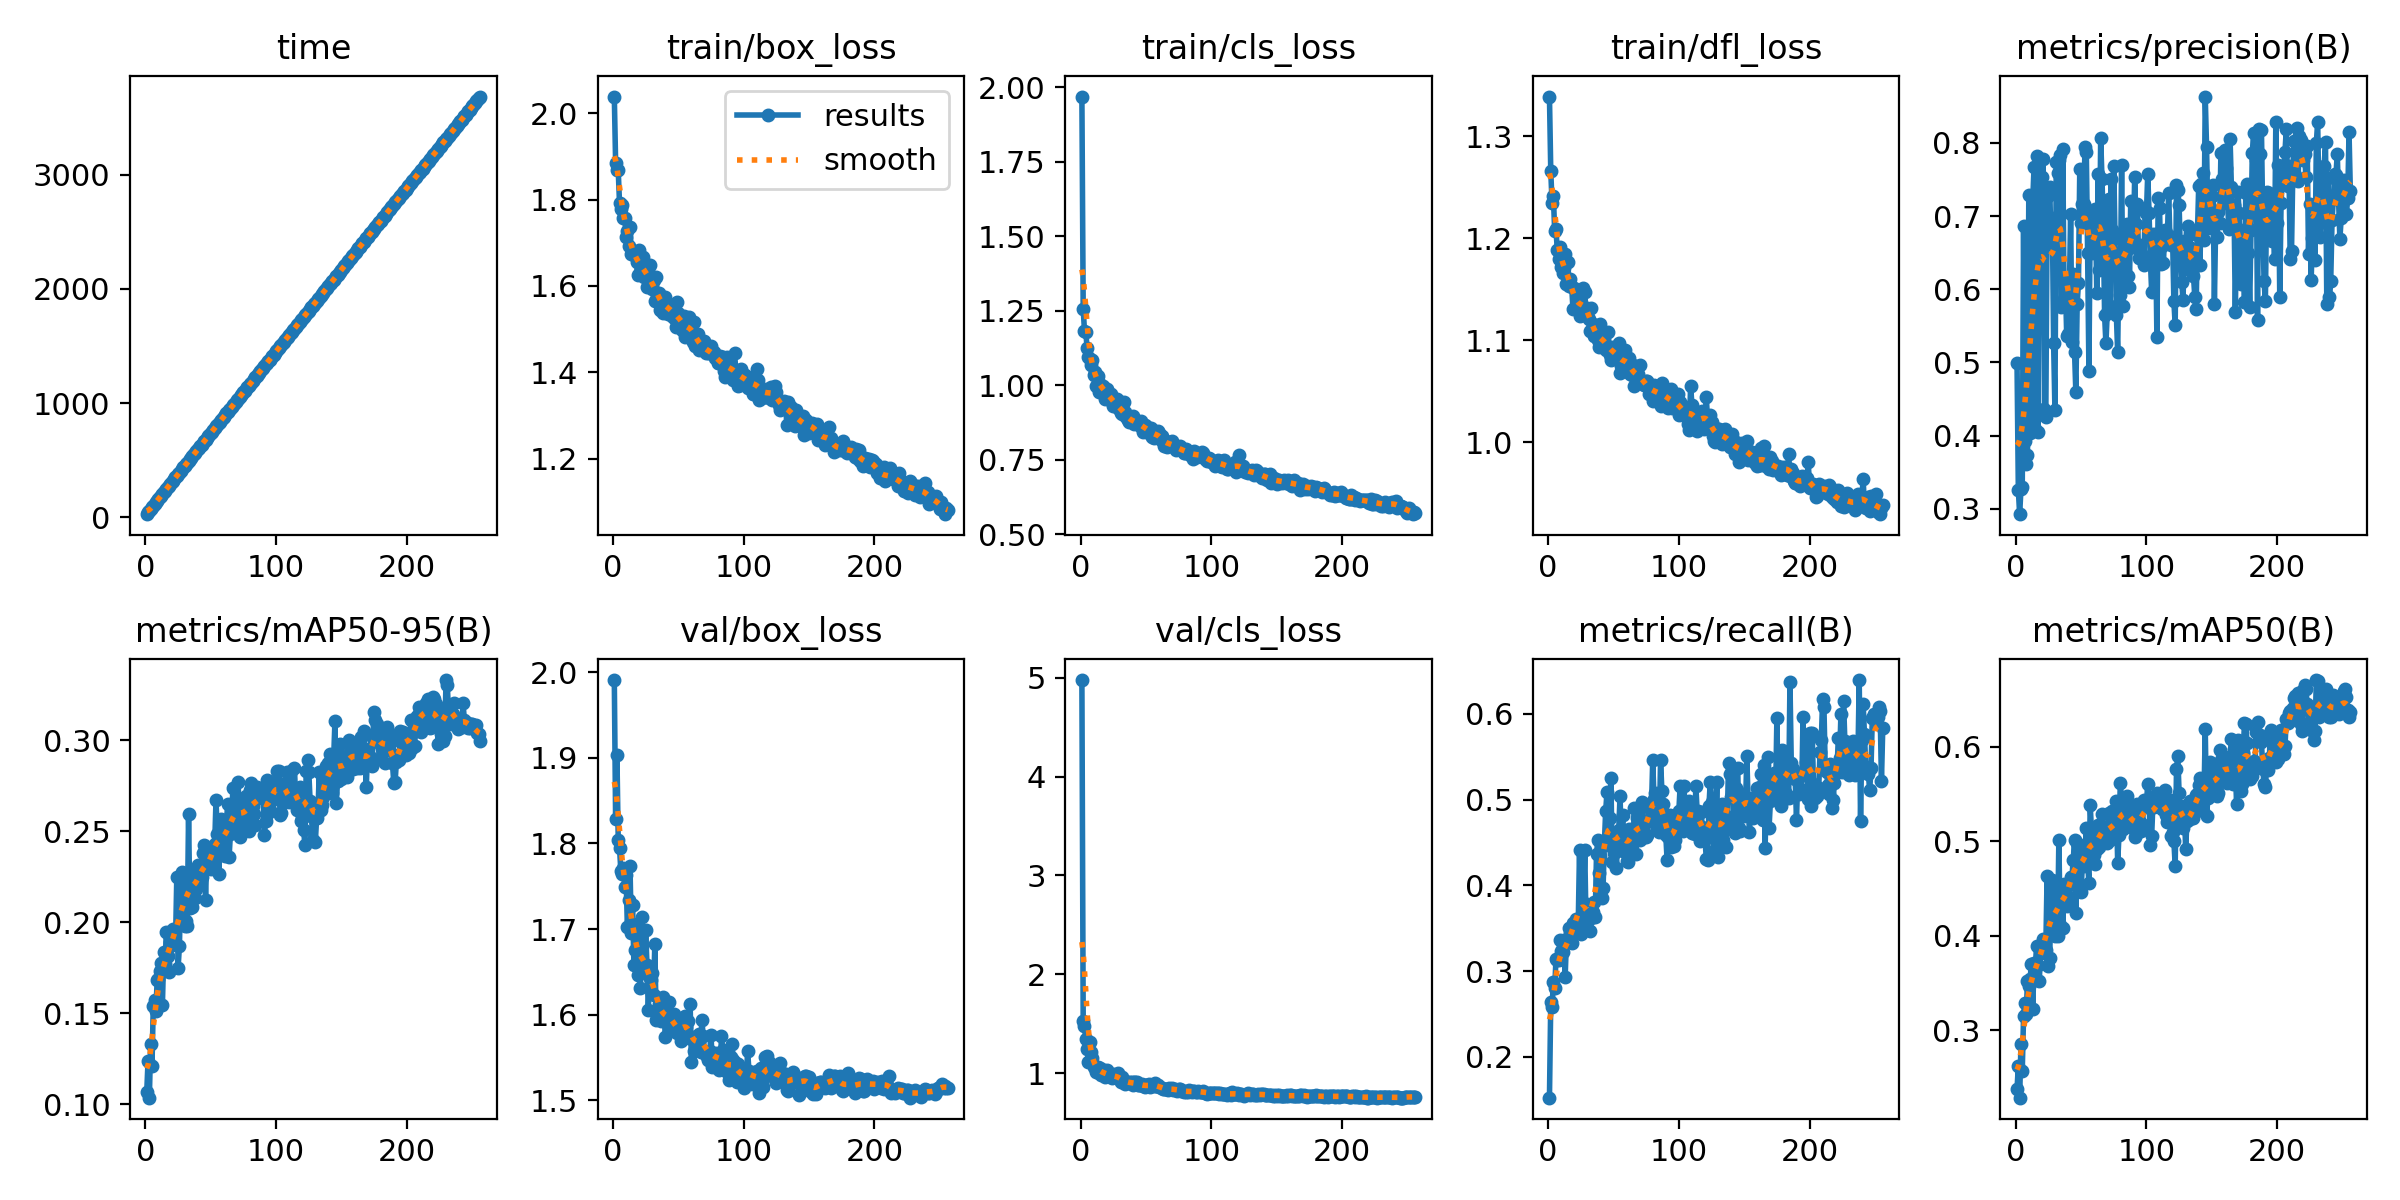
\includegraphics[width=0.9\textwidth]{thesis_final/figures/15.png}
                \caption{Deployment Results}
            \end{figure}
            
            \textbf{System Reliability:}
            \begin{table}[h]
                \tiny
                \begin{tabular}{|l|c|c|}
                    \hline
                    \textbf{Location} & \textbf{Uptime} & \textbf{Response} \\
                    \hline
                    Shahbag & 98.7\% & 245ms \\
                    Motijheel & 99.2\% & 198ms \\
                    Science Lab & 98.9\% & 223ms \\
                    \hline
                    \textbf{Average} & \textbf{98.9\%} & \textbf{222ms} \\
                    \hline
                \end{tabular}
            \end{table}
        \end{column}
    \end{columns}
\end{frame}

\section{Implementation Challenges}

\begin{frame}{Technical Challenges \& Solutions}
    \begin{columns}
        \begin{column}{0.5\textwidth}
            \textbf{Data Challenges:}
            \begin{itemize}
                \item \textcolor{red}{Challenge}: Class imbalance (0.5\% emergency vehicles)
                \item \textcolor{green}{Solution}: Data augmentation \& weighted training
            \end{itemize}
            
            \vspace{0.2cm}
            \textbf{Hardware Limitations:}
            \begin{itemize}
                \item \textcolor{red}{Challenge}: Processing power constraints
                \item \textcolor{green}{Solution}: Model optimization \& edge computing
            \end{itemize}
            
            \vspace{0.2cm}
            \textbf{Environmental Factors:}
            \begin{itemize}
                \item \textcolor{red}{Challenge}: Weather \& lighting variations
                \item \textcolor{green}{Solution}: Robust training dataset \& preprocessing
            \end{itemize}
        \end{column}
        \begin{column}{0.5\textwidth}
            \textbf{Integration Issues:}
            \begin{itemize}
                \item \textcolor{red}{Challenge}: Legacy traffic infrastructure
                \item \textcolor{green}{Solution}: Modular IoT architecture
            \end{itemize}
            
            \vspace{0.2cm}
            \textbf{Real-time Requirements:}
            \begin{itemize}
                \item \textcolor{red}{Challenge}: Sub-second response needed
                \item \textcolor{green}{Solution}: Optimized algorithms \& parallel processing
            \end{itemize}
            
            \vspace{0.2cm}
            \textbf{Scalability Concerns:}
            \begin{itemize}
                \item \textcolor{red}{Challenge}: City-wide deployment costs
                \item \textcolor{green}{Solution}: Cost-effective hardware \& phased rollout
            \end{itemize}
        \end{column}
    \end{columns}
\end{frame}

\section{Economic Impact}

\begin{frame}{Cost-Benefit Analysis}
    \begin{columns}
        \begin{column}{0.6\textwidth}
            \begin{itemize}
                \item \textbf{Annual Net Benefits}: \$8.065 million
                \item \textbf{Return on Investment}: 672\%
                \item \textbf{CO2 Reduction}: 1,245 tons annually
                \item \textbf{Fuel Savings}: 485,000 liters annually
                \item \textbf{User Satisfaction}: 87\% overall satisfaction
            \end{itemize}
        \end{column}
        \begin{column}{0.4\textwidth}
            \begin{figure}[h]
                \centering
                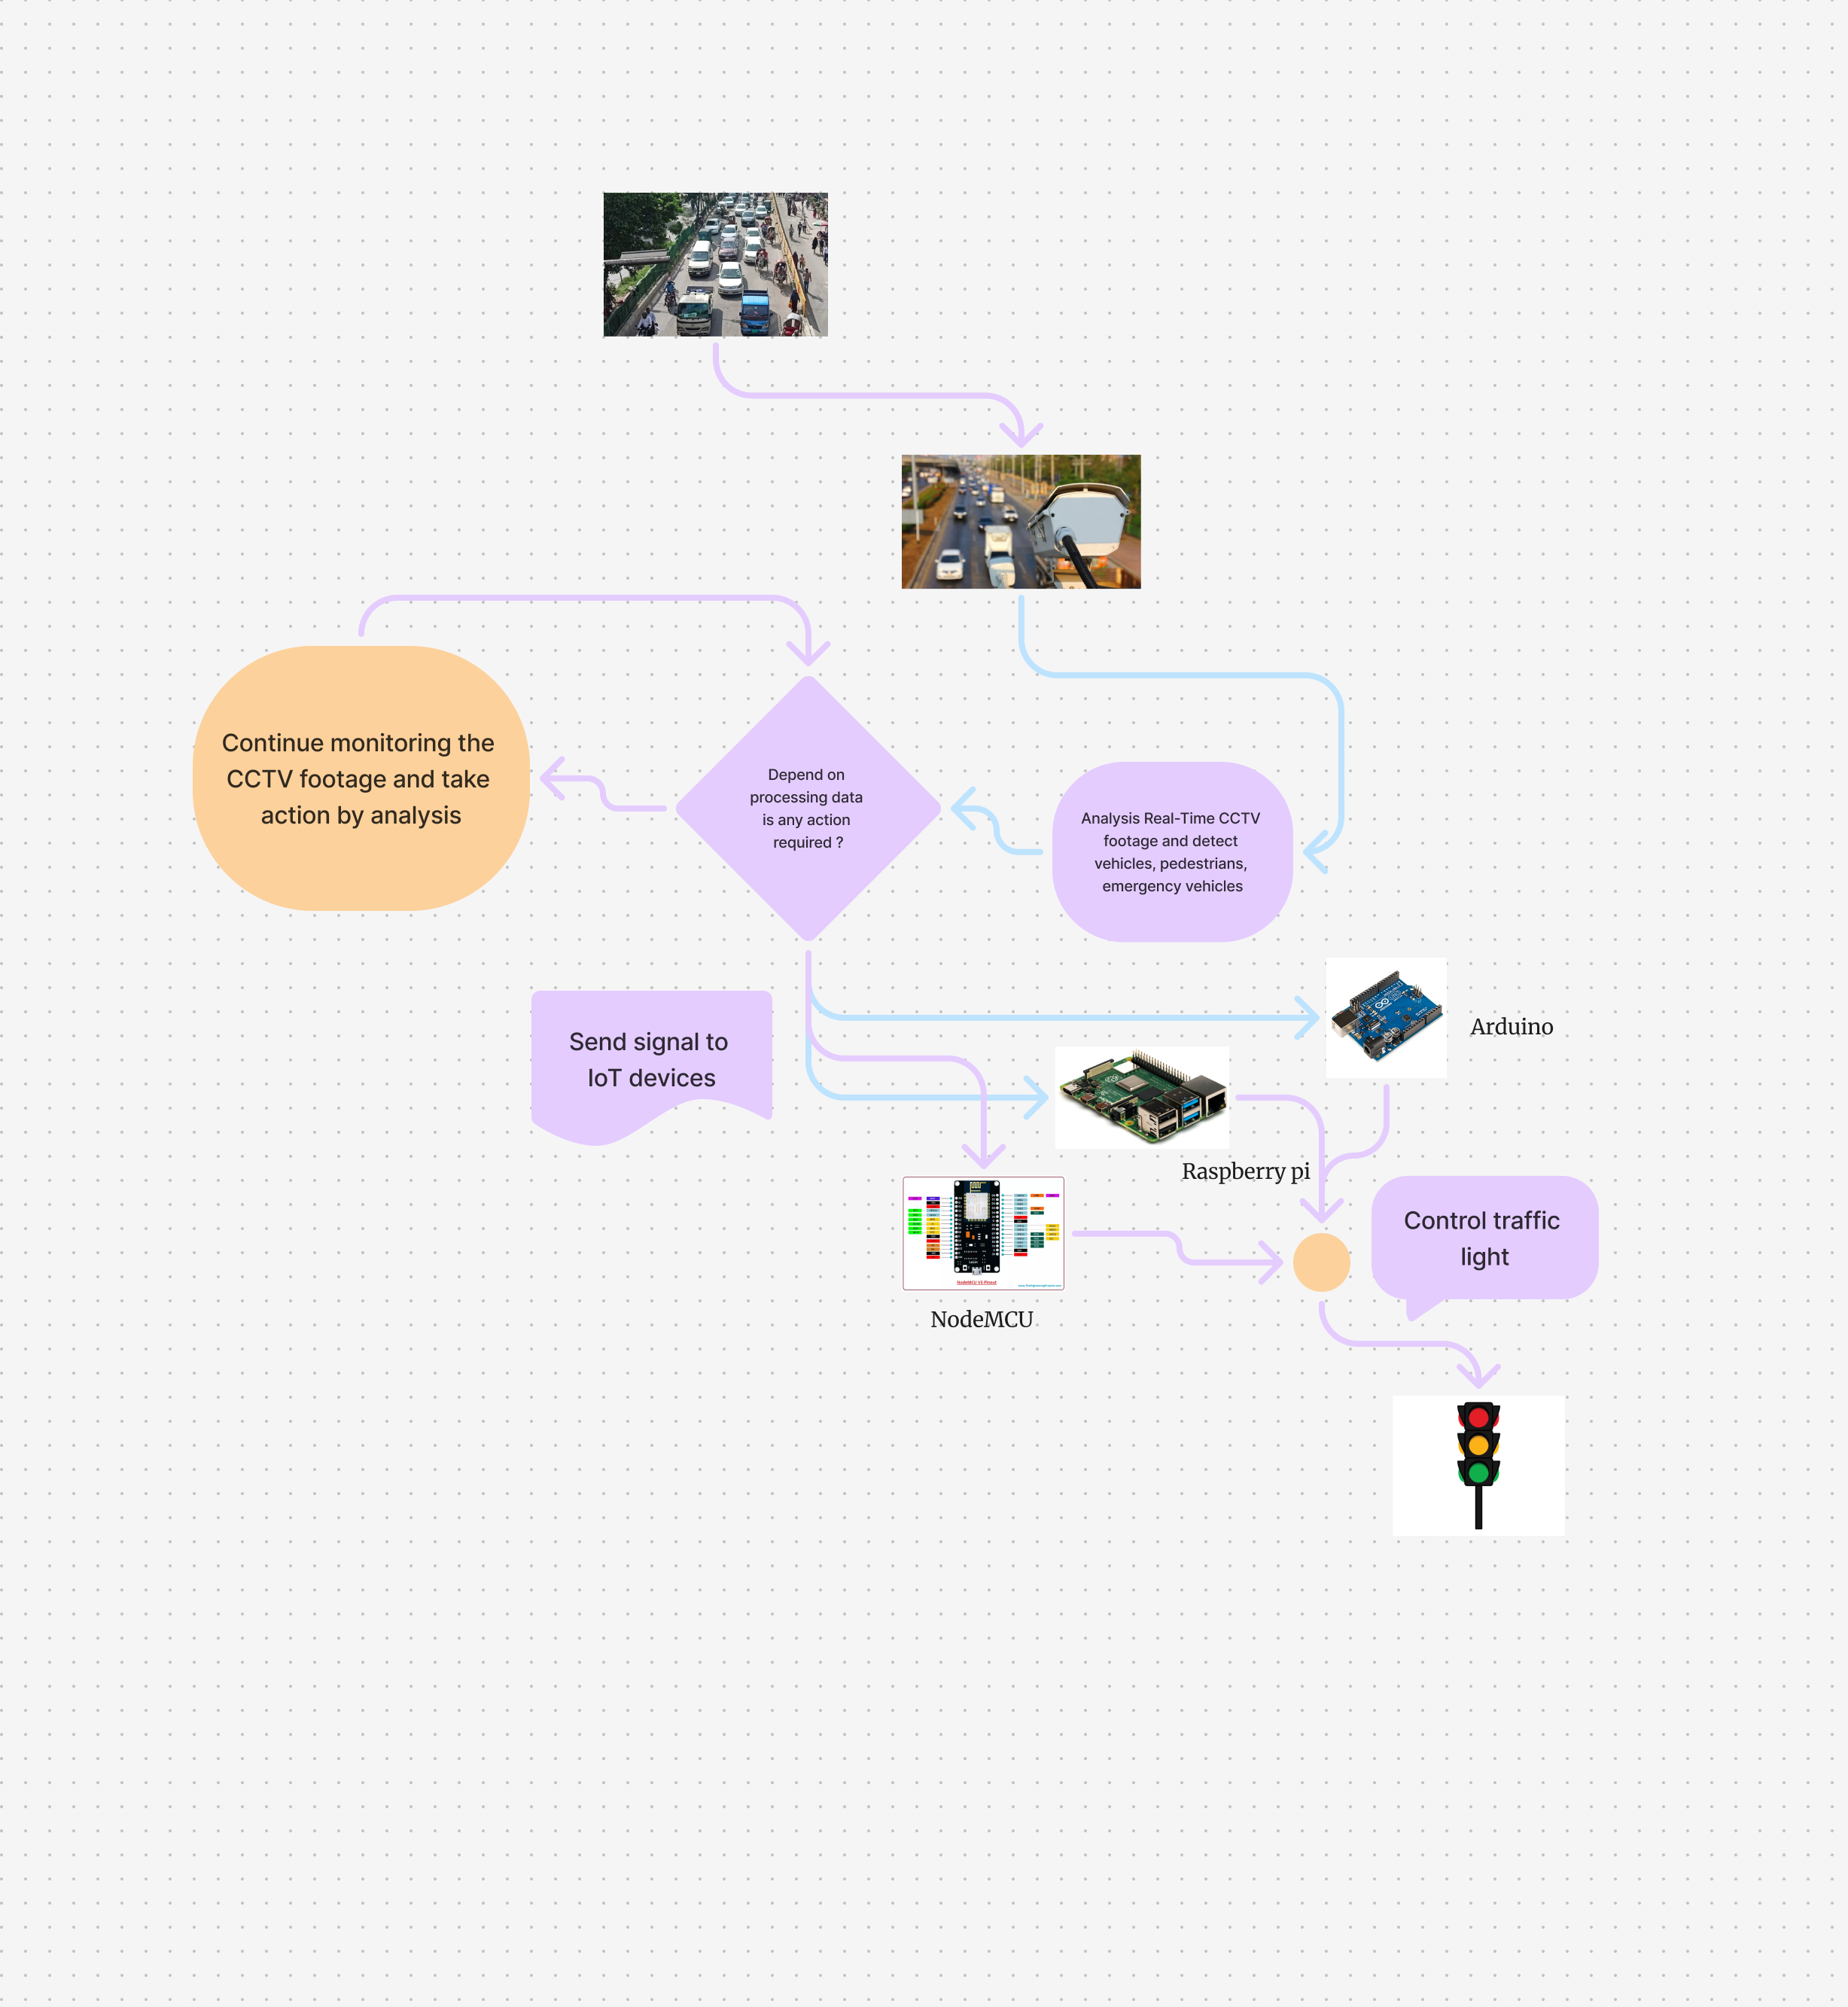
\includegraphics[width=\textwidth]{thesis_final/figures/6.png}
                \caption{\footnotesize Economic Impact Analysis}
            \end{figure}
        \end{column}
    \end{columns}
    
    \vspace{0.3cm}
    \begin{center}
        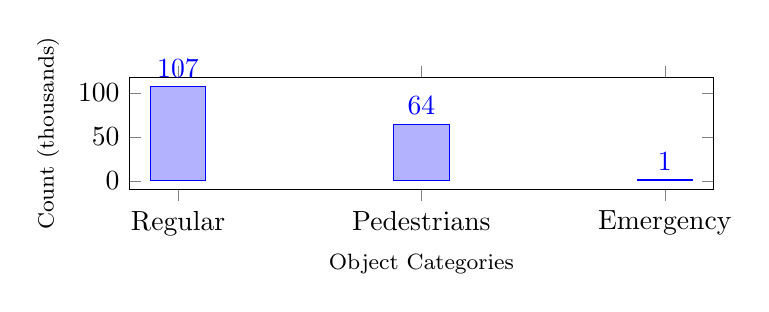
\begin{tikzpicture}
            \begin{axis}[
                ybar,
                width=9cm,
                height=3cm,
                ylabel={\footnotesize Count (thousands)},
                symbolic x coords={Regular,Pedestrians,Emergency},
                xlabel={\footnotesize Object Categories},
                xtick=data,
                nodes near coords,
                nodes near coords align={vertical},
                bar width=20pt,
                fill=lightblue!60,
                text=black,
            ]
            \addplot coordinates {
                (Regular,107)
                (Pedestrians,64)
                (Emergency,1)
            };
            \end{axis}
        \end{tikzpicture}
    \end{center}
\end{frame}

\section{Conclusions}

\begin{frame}{Key Contributions}
    \begin{enumerate}
        \item \textbf{Novel YOLOv11 Application}
        \begin{itemize}
            \item First comprehensive application for Dhaka traffic
            \item 79\% detection accuracy achieved
        \end{itemize}
        
        \item \textbf{Emergency Vehicle Prioritization}
        \begin{itemize}
            \item 56\% reduction in response times
            \item Automated detection and control
        \end{itemize}
        
        \item \textbf{Adaptive Traffic Management}
        \begin{itemize}
            \item 33\% reduction in wait times
            \item 97\% reduction in lane starvation
        \end{itemize}
        
        \item \textbf{Cost-Effective Solution}
        \begin{itemize}
            \item 672\% return on investment
            \item Commercial hardware components
        \end{itemize}
    \end{enumerate}
\end{frame}

\section{Future Work}

\begin{frame}{Future Research Directions}
    \begin{columns}
        \begin{column}{0.5\textwidth}
            \textbf{Short-term (6-12 months):}
            \begin{itemize}
                \item Emergency vehicle dataset expansion
                \item Weather-resistant algorithms
                \item Hardware optimization
                \item User interface improvements
                \item Security enhancements
            \end{itemize}
            
            \vspace{0.3cm}
            \textbf{Medium-term (1-2 years):}
            \begin{itemize}
                \item Predictive traffic modeling
                \item V2I communication integration
                \item Advanced ML algorithms
                \item Mobile app development
                \item Real-time analytics dashboard
            \end{itemize}
        \end{column}
        \begin{column}{0.5\textwidth}
            \textbf{Long-term (2-5 years):}
            \begin{itemize}
                \item City-wide deployment
                \item Smart city ecosystem integration
                \item Autonomous vehicle compatibility
                \item International standardization
                \item AI-driven traffic optimization
            \end{itemize}
            
            \vspace{0.3cm}
            \textbf{Research Opportunities:}
            \begin{itemize}
                \item Federated learning implementation
                \item Edge computing optimization
                \item Behavioral pattern analysis
                \item Environmental impact modeling
                \item Policy framework development
            \end{itemize}
        \end{column}
    \end{columns}
\end{frame}

\begin{frame}[plain]
    \begin{center}
        \vspace{1cm}
        {\Huge \textcolor{darkblue}{\textbf{Thank You!}}}
        
        \vspace{1cm}
        {\Large \textcolor{darkblue}{\textbf{Questions \& Discussion}}}
        
        \vspace{1cm}
        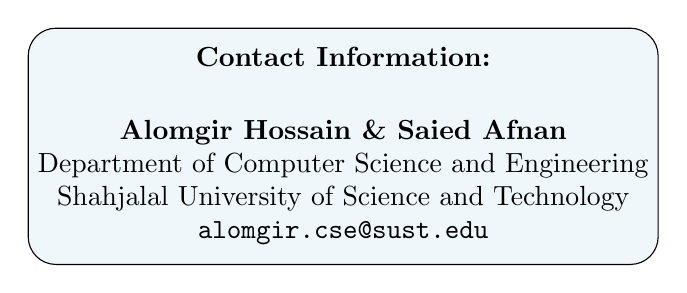
\begin{tikzpicture}
            \node[draw, rectangle, fill=lightblue!20, rounded corners=10pt, 
                  minimum width=8cm, minimum height=3cm, align=center] {
                \textbf{Contact Information:}\\[0.5cm]
                \textbf{Alomgir Hossain \& Saied Afnan}\\
                Department of Computer Science and Engineering\\
                Shahjalal University of Science and Technology\\
                \texttt{alomgir.cse@sust.edu}
            };
        \end{tikzpicture}
    \end{center}
\end{frame}

\end{document}